\documentclass[a4paper,12pt]{article}
\usepackage[chorded]{songs}
\usepackage{graphicx}
\usepackage{lmodern} % Modern font
\usepackage[utf8]{inputenc}
\usepackage{multicol}
% \usepackage[
% % set width and height to a5 width and height + 6mm
% width=154truemm, height=216truemm,
% % use any combination of these options to add different cut markings
% cam, axes, frame, cross,
% % set the type of TeX renderer you use
% pdftex,
% % center the contents
% center
% ]{crop}

\renewcommand{\familydefault}{\sfdefault}

% We use the multicol package instead of the songs package's
\songcolumns{0}
\newcommand{\nbcols}{2}

\noversenumbers
% \setlength{\songnumwidth}{0.5cm}
\renewcommand{\lyricfont}{\sffamily\small}
\renewcommand{\chorusfont}{\sffamily\small}
% \renewcommand{\snumbgcolor}{red}
\renewcommand{\printchord}[1]{{\fontsize{9}{11}\selectfont\textbf{\textsl{#1}}}}

\setlength{\cbarwidth}{1pt}
\setlength{\sbarheight}{0pt}
\setlength{\parindent}{0pt}

\setlength{\versesep}{2ex} % Increase as needed (default is usually 1ex)

\usepackage{geometry}
\geometry{
	a5paper,
	% total={170mm,257mm},
	left=12mm,
	top=10mm,
	right=10mm,
	bottom=10mm
}

% \renewcommand\printchord[1]{%
% \vbox{%
% \vskip 3pt% Add 3pt space above the chord
% \hbox{\fontsize{9}{11}\selectfont\textbf{\textsl{#1}}}%
% \vskip 0pt% Ensure proper baseline
% }%
% }

\baselineadj=-10pt plus 1pt minus 0pt
%\renewcommand{\clineparams}{
%	\baselineskip=15pt
%	\lineskiplimit=5pt
%	\lineskip=1pt
%}

\interlinepenalty=0
% \vvpenalty=0
% \ccpenalty=0
\vcpenalty=0
\cvpenalty=0
% \brkpenalty=0
\pagenumbering{gobble}

\newindex{mainindex}{idxfile}
\begin{document}
	% \begin{figure}
	% 	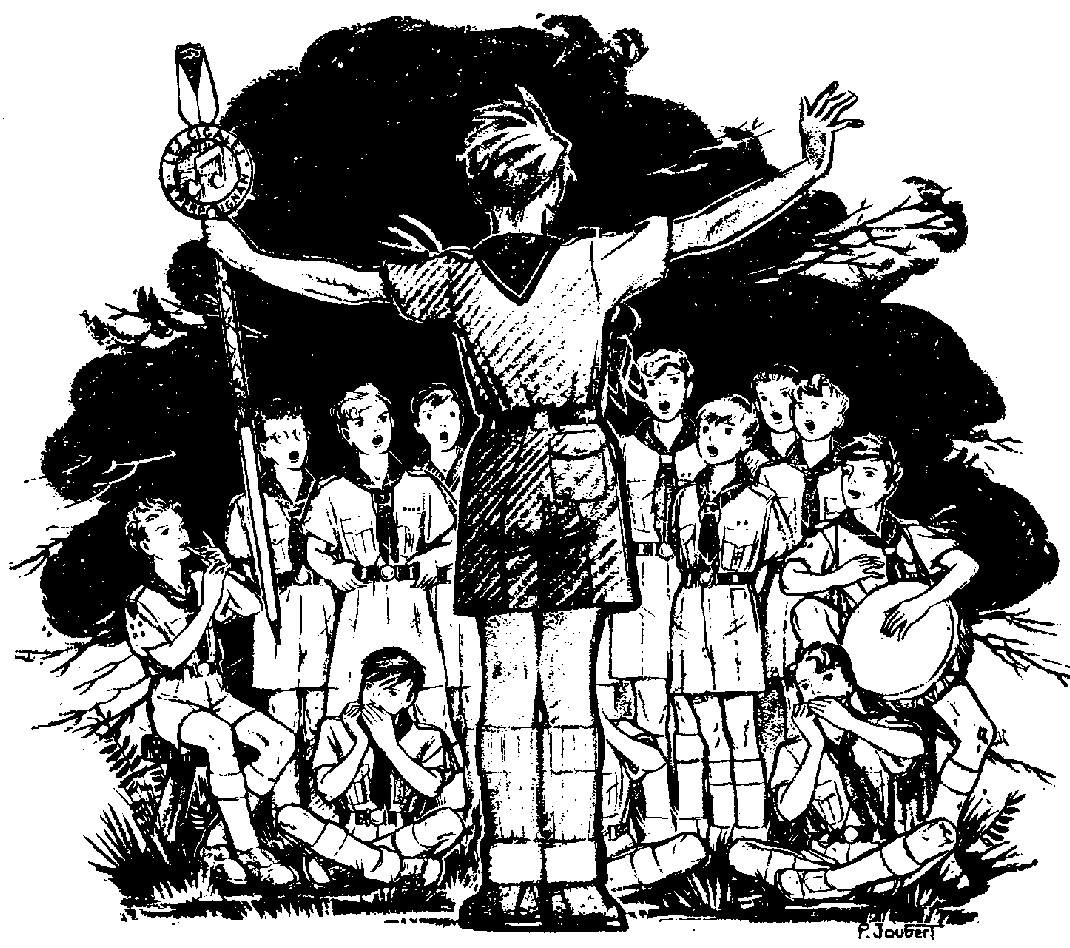
\includegraphics[width=\linewidth]{titre.jpg}
	% \end{figure}
	% \newpage

	% \showindex[2]{Index alphabétique}{mainindex}
	\begin{multicols}{\nbcols}
	\begin{songs}{}
		\beginsong{1987}[by={Calogero (2017)}]

\beginverse
Tu t'sou\[Ré]viens
Les couleurs sur les bas\[Sim]kets
Les crayons dans les cas\[La]settes
Je rembobine
Tu t'sou\[Ré]viens
Tous ces rêves plein nos disq\[Sim]uettes
À Paris c'était les S\[La]tates
198\[Mim]7 \[La] 
\endverse


\beginchorus
Il \[Ré]y a certains jours où j\[La]e reprends mon skate
Et j\[Si7]e vais faire un tour en 19\[Fa#m]87 \[Sol] \[Mim]\[La] 
Il \[Ré]y a certains jours dans \[La]lesquels je me jette
Et \[Sim7]je suis de retour en 19\[Fa#m]87 \[Sol] \[Mim]\[La] 
Tu \[Ré]sais de tous ces jours y'a \[La]rien que je regrette
Mais \[Sim7]parfois je retourne en 19\[Fa#m]8\[Sol]7, en 87
\endchorus

\beginverse
Tu t'souviens
Les survêts et les houppettes
Sabrina et 7 sur 7
Dans la cuisine c'était rien
Que 12 mois sur la planète
L'URSS, INXS
On chantait I want your sex
\endverse

\beginverse
Refrain
\endverse

\beginverse
Tu verras bien qu'un jour une chanson dans la tête
Tu l'auras à ton tour ton 1987
Tu verras bien qu'un jour une chanson dans la tête
Tu l'auras à ton tour ton 1987
C'est tout ce que je te souhaite
Tu l'auras à ton tour ton 1987
C'est tout ce que je te souhaite
Tu l'auras à ton tour ton 1987
C'est tout ce que je te souhaite
Tu l'auras à ton tour ton 1987
Tu t'souviens
\endverse

\endsong
\beginsong{99 Luftballons}[by={Nena (1983)}]

\beginverse
\[Ré]Hast du etwas \[Mim]Zeit für mich?
Dann \[Sol]singe ich ein \[La]Lied für dich
Von \[Ré]99 \[Mim]Luftballons
Auf \[Sol]ihrem Weg zum \[La]Horizont
\[Ré]Denkst du vielleicht \[Mim]g'rade an mich
Dann \[Sol]singe ich ein \[La]Lied für dich
Von \[Ré]99 \[Mim]Luftballons
Und \[Sol]das sowas von \[La]sowas kommt
\endverse

\beginverse
99 Luftballons
Auf ihrem Weg zum Horizont
Hielt man für UFOs aus dem All
Darum schickte ein General
Eine Fliegerstaffel hinterher
Alarm zu geben, wenn es so wäre
Dabei waren da am Horizont
Nur 99 Luftballons
\endverse

\beginverse
99 Düsenflieger
Jeder war ein großer Krieger
Hielten sich für Captain Kirk
Das gab ein großes Feuerwerk
Die Nachbarn haben nichts gerafft
Und fühlten sich gleich angemacht
Dabei schoss man am Horizont
Auf 99 Luftballons
\endverse

\beginverse
99 Kriegsminister
Streichholz und Benzinkanister
Hielten sich für schlaue Leute
Witterten schon fette Beute
Riefen Krieg und wollten Macht
Mann, wer hätte das gedacht
Dass es einmal soweit kommt
Wegen 99 Luftballons
\endverse

\beginverse
99 Jahre Krieg
Ließen keinen Platz für Sieger
Kriegsminister gibt es nicht mehr
Und auch keine Düsenflieger
Heute ziehe ich meine Runden
Sehe die Welt in Trümmern liegen
Habe einen Luftballon gefunden
Denke an dich und lasse ihn fliegen
\endverse

\endsong
\beginsong{À nos souvenirs}[by={Trois cafés gourmands (2018)}]

(Capo IV)

\beginverse
Comment puis-je oubl\[Lam]ier
Ce coin de para\[Fa]dis?
Ce petit bout de \[Do]terre
Où vit encore mon \[Sol]père
\endverse

\beginverse
Comment pourrais-je \[Lam]faire
Pour me séparer \[Fa]d'elle?
Oublier qu'on est \[Do]frères
Belle Corrèze char\[Sol]nelle
Oublier ce ma\[Lam]tin que tu es par\[Fa]isien
Que t'as de l'eau dans le \[Do]vin
Que tu es parti \[Sol]loin
\endverse

\beginverse
Ce n'était pas ma faute
On joue des fausses notes
On se trompe de chemin
Et on a du chagrin
On se joue tout un drame
On a des vagues à l'âme
Tu as du mal au cœur
Tu as peur du bonheur
\endverse

\beginverse
Acheter des tableaux
Et des vaches en photo
C'est tout ce que t'as trouvé
Pour te la rappeler
Vous me trouvez un peu con
N'aimez pas ma chanson
\endverse

\beginverse
Vous me croyez bizarre
Un peu patriotard
Le fruit de ma réflexion
Ne touchera personne
Si vos pas ne résonnent
Jamais dans ma région
\endverse

\beginverse
C'est pire qu'une religion
Au-delà d'une confession
Je l'aime à en mourir
Pour le meilleur et pour le pire
Et si je monte au ciel
Il y aura peut-être Joël
\endverse

\beginverse
Guillaume et Jeremy
Et mon cousin Piedri
Yoan sera en voyage
Dans un autre pays
Allez fais tes bagages
Viens rejoindre tes amis
\endverse

\beginverse
On veut du Clody Musette
À en perdre la tête
On veut un dernier Chabrol
Un petit coup de gnôle
Les yeux de nos grands-mères
La voix de nos grands-pères
L'odeur de cette terre
Vue sur les Monédières
\endverse

\beginverse
C'est pire qu'un testament
Au-delà d'une confidence
On est des petits enfants
De ce joli coin de France
Enterrez-nous vivants
Bâillonnés s'il le faut
Mais prenez soin avant
De remplir notre jabot
\endverse

\beginverse
La relève est pour toi
Notre petit Lucas
On t'laisse en héritage la piste
Nous, on dégage
Le temps nous a gâtés
On en a bien profité
On a des souvenirs en tête
Ce soir, faisons la fête
\endverse


\beginchorus
Acceptez ma rengaine
Elle veut juste dire “je t'aime”
Soyez sûr, j'en suis fier
J'ai la Corrèze en cathéter
D'être avec vous ce soir
J'ai le cœur qui pétille
Mimi, sers-nous à boire
On a les yeux qui brillent
\endchorus

\beginverse
Papayapapa, papayapapa, papayapapa
Paya, papayapapa (4x)
\endverse

\beginverse
Refrain
\endverse

\endsong
\beginsong{L'agriculteur}[by={Ridan (2003)}]

\beginverse
J'allume mon p\[Lam]oste de tél\[Do]é
Pour admir\[Sol]er ce qu'il s'y p\[Lam]asse
Un milliard\[Fa]aire s'envoie en l\[Rém]'air
Toute l'at\[Mim]mosphère pour voir l'esp\[Lam]ace
J'troque son bol d\[Lam]'air et sa cuil\[Do]lère
Contre un p'tit v\[Sol]erre sur ma ter\[Lam]rasse
J'en ai ras-le-b\[Fa]ol de tout ce bét\[Rém]on
J'ai la fol\[Mim]ie des grands esp\[Lam]aces
\[Lam]\[Do]\[Sol]\[Lam]J'en ai ras-le-b\[Fa]ol de tout ce bét\[Rém]on
J'ai la fol\[Mim]ie des grands esp\[Lam]aces
Mais qu'est-ce qui s\[Lam]e passe dans nos p'tites t\[Do]êtes?
On s'entasse t\[Sol]ous comme des sard\[Lam]ines
Dans les grosses b\[Fa]oîtes que l'on cons\[Rém]erve
Le p'tit pois\[Mim]son doit suivre sa l\[Lam]igne
\[Lam]\[Do]\[Sol]\[Lam] Dans les grosses b\[Fa]oîtes que l'on cons\[Rém]erve
Le p'tit pois\[Mim]son doit suivre sa l\[Lam]igne
\endverse

\beginchorus
Et puis m\[Lam]erde! J'ai décid\[Do]é de vivre l\[Sol]oin sur la col\[Lam]line
Vivre s\[Fa]eul dans une mais\[Rém]on avec la v\[Mim]ue sur ma rais\[Lam]on
J'préfère vivre p\[Lam]auvre avec mon â\[Do]me, que vivre r\[Sol]iche avec la l\[Lam]eur
Et si le b\[Fa]lé m'file du bonh\[Rém]eur, j'me ferais p\[Mim]'têt' agricult\[Lam]eur 
\[Lam]\[Do]\[Sol]\[Lam] Et si le b\[Fa]lé m'file du bonh\[Rém]eur, j'me ferais p\[Mim]'têt' agricult\[Lam]eur
\endchorus

\beginverse
Y a trop d'feux rouges dans les grandes villes
J'ai préféré me mettre au vert
J'ai plus d'bonheur à vivre en paix
Que d'm'admirer au fond d'un verre
J'boirai l'eau saine de mon ruisseau
Plutôt qu'l'eau sale du fond de la Seine
Chargée en plomb et en histoire
Que la surface ne laisse plus voir
Chargée en plomb et en histoire
Que la surface ne laisse plus voir
J'ferai des bornes pour m'éloigner
Pour m'retrouver face au miroir
Juste une seconde de vérité
Pour qu'mon passé coule sous les ponts
J'ferai des bornes pour m'éclipser
Pour m'retrouver face à que dalle
Juste une seconde de vérité
Pour contempler ce qu'on est tous
\endverse

\beginchorus
Refrain
\endchorus

\beginverse
Ça fait longtemps que j'n'ai plus vu
Ce coin d'soleil à l'horizon
Ça fait longtemps que j'l'attendais
La petite lueur de la raison
Une petite chanson au clair de lune
Pour réchauffer le cœur de pierre
Le grand retour à l'essentiel
Le feu de bois éclaire le ciel
Le grand retour à l'essentiel
Le feu de bois éclaire le ciel
La mélodie de la nature
Reprend ses droits sur la folie
C'est toute la vie qui nous observe
Que l'on oublie au fil du temps
La mélodie, celle de la vie
Que l'on consume à chaque instant
Tous nos acquis s'écrasent au sol
Et j'ai choisi la clé des champs
Tous nos acquis s'écrasent au sol
Et j'ai choisi la clef des champs
\endverse

\beginchorus
Refrain (bis)
\endchorus

\beginverse
J'allume mon \[Sim]poste de té\[Ré]lé
Pour admi\[La]rer ce qu'il s'y \[Sim]passe
Un milliar\[Sol]daire s'envoie en \[Mim]l'air
Toute l'at\[Fa#m]mosphère pour voir l'es\[Sim]pace
J'troque son bol \[Sim]d'air et sa cui\[Ré]llère
Contre un p'tit \[La]verre sur ma te\[Sim]rrasse
J'en ai ras-le-\[Sol]bol de tout ce bé\[Mim]ton
J'ai la fol\[Fa#m]ie des grands es\[Sim]paces
\[Sim] \[Ré]\[La] J'\[Sim]en ai ras-le-bol de \[Sol] tout ce béto\[Mim]n
J'ai la fol\[Fa#m]ie des grands esp\[Sim]aces
Mais qu'est-ce qui \[Sim]se passe dans nos p'tites \[Ré]têtes?
On s'entasse \[La]tous comme des sar\[Sim]dines
Dans les grosses \[Sol]boîtes que l'on con\[Mim]serve
Le p'tit pois\[Fa#m]son doit suivre sa \[Sim]ligne
\[Sim] \[Ré]\[La]Dans \[Sim] les grosses boîtes q\[Sol]ue l'on conserv\[Mim]e
Le p'tit poisson d\[Fa#m]oit suivre sa lign\[Sim]e
\endverse


\beginchorus
Et puis \[Sim]merde! J'ai déci\[Ré]dé de vivre \[La]loin sur la co\[Sim]lline
Vivre \[Sol]seul dans une mai\[Mim]son avec la v\[Fa#m]ue sur ma rai\[Sim]son
J'préfère vivre \[Sim]pauvre avec mon \[Ré]âme, que vivre \[La]riche avec la \[Sim]leur
Et si le \[Sol]blé m'file du bon\[Mim]heur, j'me ferais p\[Fa#m]'têt' agricul\[Sim]teur
\[Sim] \[Ré]\[La] Et \[Sim]si le blé m'file \[Sol] du bonheur, j'me \[Mim] ferais p'têt'\[Fa#m] agriculteu\[Sim]r
\endchorus

\beginverse
Y a trop d'feux rouges dans les grandes villes
J'ai préféré me mettre au vert
J'ai plus d'bonheur à vivre en paix
Que d'm'admirer au fond d'un verre
J'boirai l'eau saine de mon ruisseau
Plutôt qu'l'eau sale du fond de la Seine
Chargée en plomb et en histoire
Que la surface ne laisse plus voir
Chargée en plomb et en histoire
Que la surface ne laisse plus voir
J'ferai des bornes pour m'éloigner
Pour m'retrouver face au miroir
Juste une seconde de vérité
Pour qu'mon passé coule sous les ponts
J'ferai des bornes pour m'éclipser
Pour m'retrouver face à que dalle
Juste une seconde de vérité
Pour contempler ce qu'on est tous
\endverse

\beginverse
Refrain
\endverse

\beginverse
Ça fait longtemps que j'n'ai plus vu
Ce coin d'soleil à l'horizon
Ça fait longtemps que j'l'attendais
La petite lueur de la raison
Une petite chanson au clair de lune
Pour réchauffer le cœur de pierre
Le grand retour à l'essentiel
Le feu de bois éclaire le ciel
Le grand retour à l'essentiel
Le feu de bois éclaire le ciel
La mélodie de la nature
Reprend ses droits sur la folie
C'est toute la vie qui nous observe
Que l'on oublie au fil du temps
La mélodie, celle de la vie
Que l'on consume à chaque instant
Tous nos acquis s'écrasent au sol
Et j'ai choisi la clé des champs
Tous nos acquis s'écrasent au sol
Et j'ai choisi la clef des champs
\endverse

\beginverse
Refrain (bis)
\endverse

\endsong
\beginsong{Ah les crocodiles !}[by={Jacques Offenbach (1856), Julien Doré (2024)}]

\beginverse
\[Ré]Un crocodile s'en allant à la \[La]guerre
\[Mi]Disait au revoir \[Mi7]à ses petits \[La]enfants
\[Ré]Traînant ses pieds, ses pieds dans la pouss\[La]ière
\[Mi]Il s'en allait combattre les élé\[La7]phants
\endverse


\beginchorus
\[Ré]Ah' les crocrocros, les crocrocros, les croco\[La7]diles
Sur les bords du Nil, ils sont partis, n'en parlons \[Ré]plus
(bis)
\endchorus

\beginverse
Il fredonnait une marche militaire
Dont il mâchait les mots à grosses dents
Quand il ouvrait la gueule tout entière
On croyait voir ses ennemis dedans
\endverse

\beginverse
Il agitait sa grand queue à l'arrière
Comme s'il était d'avance triomphant
Les animaux devant sa mine altière
Dans les forêts s'enfuyaient tout tremblants.
\endverse

\beginverse
Un éléphant parut et sur la terre
Se prépara ce combat de géants
Mais près de là courait une rivière
Le crocodile s'y jeta subitement
\endverse

\beginverse
Et tout rempli d'une crainte salutaire
Il s'en retourna vers ses petits enfants
Notre éléphant, d'une trompe plus fière
Voulut alors accompagner ce chant.
\endverse

\endsong
\beginsong{Aïcha}[by={Khaled (1996)}]

\beginverse
Capo III
\[Mim] Comme \[Do]si je n'ex\[Sol]istais \[Ré]pas
\[Mim] Elle e\[Do]st passée à côt\[Sol]é de \[Ré]moi
\[Mim] Sans un \[Do]regard, \[Sol]reine de \[Ré]Saba
\[Mim] J'ai \[Do]dit “Aïcha, prends, tout \[Sol]est pour t\[Ré]oi”
\endverse

\beginverse
Voici les perles, les bijoux
Aussi l'or autour de ton cou
Les fruits bien mûrs au goût de miel
Ma vie, Aïcha, si tu m'aimes
J'irai où ton souffle nous mène
Dans les pays d'ivoire et d'ébène
J'effacerai tes larmes, tes peines
Rien n'est trop beau pour une si belle, oh!
\endverse


\beginchorus
\[Mim] Aïc\[Do]ha, Aïcha, \[Sol]écoute-m\[Ré]oi
\[Mim] Aïc\[Do]ha, Aïcha, \[Sol]t'en va p\[Ré]as
\[Mim] Aïc\[Do]ha, Aïcha, r\[Sol]egarde-m\[Ré]oi
\[Mim] Aïc\[Do]ha, Aïcha, r\[Sol]éponds-m\[Ré]oi
\endchorus

\beginverse
Je dirai les mots, les poèmes
Je jouerai les musiques du ciel
Je prendrai les rayons du soleil
Pour éclairer tes yeux de reine, oh!
\endverse

\beginverse
Refrain
\endverse

\beginverse
\[Misus4] \[Lam]Elle a dit, “Garde tes t\[Fa]résors
\[Lam]Moi, je vaux mieux que tout ç\[Fa]a
\[Rém] Des barreaux sont des barreaux, même \[Sol]en or
Je veux les \[Misus4]mêmes dr\[Mi]oits que t\[Lam]oi
\[Fa] Et du respect pour chaque j\[Rém]our
\[Rém]Moi, je ne veux que de l'\[Misus4]amour”\[Mi]
\endverse

\beginverse
\[Mim] Comme \[Do]si je n'ex\[Sol]istais \[Ré]pas
Elle est passée à côté de moi
Sans un regard, reine de Saba
J'ai dit “Aïcha, prends, tout est pour toi”
\endverse

\endsong
\beginsong{L'aigle noir}[by={Barbara (1970)}]

\beginverse
\[Ré]Un beau jour ou peut-être \[La]une nuit
\[Mim]Près d'un lac je m'étais endormie
Quand soudain semblant crever le ciel
Et venant de nulle part
Surgit un aigle noir
\endverse

\beginverse
Lentement les ailes déployées
Lentement je le vis tournoyer
Près de moi dans un bruissement d'ailes
Comme tombé du ciel
L'oiseau vint se poser
\endverse

\beginverse
Il avait les yeux couleur rubis
Et les plumes couleur de la nuit
A son front, brillant de mille feux
L'oiseau roi couronné
Portait un diamant bleu
\endverse

\beginverse
De son bec il a touché ma joue
Dans ma main il a glissé son cou
C'est alors que je l'ai reconnu
Surgissant du passé
Il m'était revenu
\endverse

\beginverse
Dis, l'oiseau, oh dis, emmène-moi
Retournons au pays d'autrefois
Comme avant dans mes rêves d'enfant
Pour cueillir en tremblant
Des étoiles, des étoiles
\endverse

\beginverse
Comme avant dans mes rêves d'enfant
Comme avant sur un nuage blanc
Comme avant, allumer le soleil
Etre faiseur de pluie
Et faire des merveilles
\endverse

\beginverse
L'aigle noir dans un bruissement d'ailes
Prit son vol pour regagner le ciel
\endverse

\beginverse
Un beau jour ou peut-être une nuit
Près d'un lac je m'étais endormie
Quand soudain semblant crever le ciel
Et venant de nulle part
Surgit un aigle noir
\endverse

\endsong
\beginsong{Allô le monde}[by={Pauline (2007)}]

(Capo I)

\beginverse
Il pa\[Lam]raît que les nouv\[Fa]elles ne \[Do]sont pas si b\[Sol]onnes
Que le mora\[La]l des\[Fa]cend
Et que l\[Do]es forces t'aband\[Sol]onnent
J'en\[Lam]tends
Tous les \[Fa]gens
Par\[Do]ler de tes his\[Sol]toires
Que l'ave\[Lam]nir qui t'at\[Fa]tend
Se joue sur le \[Do]fil du ra\[Sol]soir
Qu'en est-\[Fa]il de l'a\[Sol]mour?
Des \[Fa]larmes et de la \[Sol]peine?
De la \[Fa]vie de tous les \[Sol]jours?
Et d\[Fa]e la paix \[Sol]sereine?
\endverse


\beginchorus
Allô le \[Lam]monde \[Fa] 
\[Lam]Est-ce que tout va b\[Sol]ien?
Allô le mon\[Lam]de \[Fa] 
Je \[Lam]n'y comprends plus \[Sol]rien
Allô le mon\[Lam]de \[Fa] 
\[Lam]Prends soin de \[Sol]toi
Allô le mon\[Lam]de \[Fa] 
Ne te laisse \[Lam]pas aller \[Sol] 
Comme \[Lam]ç\[Fa]a\[Lam] \[Sol]
\[Sol]Comme \[Lam]ç\[Fa]a\[Lam] \[Sol]
\endchorus

\beginverse
Quel est le nom du mal dont tu subis la fièvre
Les étranges idéaux, les hystéries funèbres?
Dis-moi ce que je peux faire de ma petite place
Quels sont les actes et les mots qui peuvent t'aider à faire face?
Pousser à la révolte
Pour faire le premier pas
Semer pour qu'on récolte
Pour crier mon effroi
\endverse

\beginverse
\[Lam]Allô le \[Rém]monde
\[Fa] Allô le \[Sol]monde
\[Lam]Allô le \[Rém]mond\[Fa]e\[Sol] 
Allô le monde
Allô le monde
\endverse

\beginverse
Allô le monde
Est-ce que tout va bien?
Allô le monde
Allô le monde
Prends soin de toi
Allô le monde
Le monde, le monde, le monde, le monde
Le monde, le monde, le monde, le monde
Allô le monde
Allô le monde, le monde
\endverse

\endsong
\beginsong{L'alphabet scout}[by={Traditionnel}]

\beginverse
Un j\[Do]our la troupe campa, A \[Sol]A A
La pluie se mit à tomber, \[Sol7]B B \[Do]B
L'orage a tout cassé, C C \[Sol]C
Faillit nous inon\[Do]der, A \[Sol]B C \[Do]D
\endverse

\beginverse
Le chef s'est écrié, E E E
A son adjoint Joseph, F F F
Fais-nous vite à manger, G G G
Les scouts sont sous la bâche E F G H
\endverse

\beginverse
Les pinsons dans leur nid, I l I
Les cerfs dans leur logis, J J J
Chahutent, quel fracas, K K K
Avec les hirondelles, I J K L
\endverse

\beginverse
Joseph nous fit d'la crème, M M M
Et du lapin d'Garenne, N N N
Et même du cacao, O O O
Mes amis quel souper, M N O P
\endverse

\beginverse
Soyez bien convaincus, QQ Q
Que la vie au grand air, R R R
Fortifie la jeunesse, S S S
Et lui rend la santé, Q R S T
\endverse

\beginverse
Maint'nant qu'il ne pleut plus, U U U
Les scouts peuvent se sauver, V V V
Le temps est au beau fixe, X X X
Plus besoin qu'on les aide, U V XZ
\endverse

\endsong
\beginsong{L'amour brille sous les étoiles}[by={Elton John, Tim Rice \- Le Roi Lion (1994)}]

\beginverse
\[Sol] C'est terrible c'est aff\[Ré]reux \- Quoi?
Et \[Sol]ils se moquent de \[Ré]tout \- Qui?
L'a\[Sol]mour s'amène et \[Sim]nous pauvres pouilleux
Ils \[Mim]nous jettent tous les \[La]deux \- Oh !
Sous \[Sol]les diamants des \[Ré]étoiles
Quel \[Sol]magique uni\[Ré]vers
Mais…\[Sol] Dans cette ro\[Sim]mantique atmosp\[Sol]hère
Ça \[Fa]sent mauvais dans \[Ré]l'air
\endverse

\beginverse
\[Sol] L'amour b\[Ré]rille sous \[Mim]les étoi\[Do]les
\[Sol] D'une étran\[Do]ge lumiè\[Ré]re
\[Do] La terre en\[Sol]tière
En \[Mim]parfaite h\[Do]armonie
Vit \[Lam]un mo\[Fa]ment ro\[Ré]yal
\endverse

\beginverse
Je voudrais lui dire je t'aime
Mais comment lui avouer
Mon secret mes problèmes
Impossible
Elle serait trop blessée
\endverse

\beginverse
Quel lourd secret cache-t-il
Derrière tant de ranceur
Moi je sais qu'il est ce roi en exil
Qui règne dans mon coeur
\endverse

\beginverse
L'amour brille sous les étoiles
D'une étrange lumière
La terre entière
En parfaite harmonie
Vit sa plus belle histoire
\endverse

\beginverse
L'amour brille sous les étoiles
Illuminant leurs coeurs
Sa lumière éclaire à l'infini
Un sublime espoir
\endverse

\beginverse
S'ils s'enfuient vers
Leur rêve ce soir
Dans leur folle ronde
Si notre ami nous dit au revoir
Nous serons seuls au monde
\endverse

\endsong
\beginsong{Amour censure*}[by={Hoshi (2020)}]

\beginverse
\[Do] Au pla\[Sol]card mes senti\[Ré]ments
Surtout ne rien d\[Mim]ire, et faire semb\[Do]lant
Être à \[Sol]part, un peu penc\[Ré]hant
Au bout du nav\[Mim]ire, je coule doucement
\endverse

\beginverse
\[Do] Maman désolée, j'vais pas te mentir
\[Sol] C'est dur d'effacer tout ce qui m'attire
\[Ré] Un peu dépassée par tous mes dé\[Mim]sirs
\[Do] Papa c'est vrai, j'ai poussé de travers
\[Sol] J'suis une fleur qui se bat entre deux pierres
\[Ré] J'ai un cœur niqué par les bonnes maniè\[Mim]res
\endverse


\beginchorus
\[Do] Est-ce qu'on va un jour en finir
\[Sol] Avec la haine et les injures
\[Ré] Est-ce que quelqu'un viendra leur dire
\[Mim] Qu'on s'aime et que c'est pas impur
\[Do] Pour pas que j'pense à en finir
\[Sol] Vos coups m'ont donné de l'allure
\[Ré] Pour le meilleur et pour le pire
\[Mim] J'prendrai d'sa main un jour c'est sûr
\endchorus

\beginverse
\[Sol] Il n'y a pas d'amour cen\[Ré]sure
\[Mim] Il n'y a que d'l'amour sin\[Do]cère
\[Sol] Il n'y a pas d'amour cen\[Ré]sure
\[Mim] Il n'y a que d'l'amour sin\[Do]cère
\endverse

\beginverse
Travestir qui je suis vraiment
Faire taire la rumeur
Les mots sont tranchants
Se mentir à s'arracher les dents
Ils cherchent un docteur
On souffre sans être souffrants
\endverse

\beginverse
Maman désolée, j'ai pris tes calmants
C'est pas que j'voulais partir, mais c'est violent
J'voulais juste dormir un peu plus longtemps
Papa t'inquiète j'ai appris à courir
Moi aussi j'veux une famille à nourrir
On s'en fout près de qui j'vais m'endormir
\endverse

	Refrain(2x)

\beginverse
Il n'y a pas d'amour censure
Il n'y a que d'l'amour sincère
(Les enfants, c'est pour un homme et une femme)
Il n'y a pas d'amour censure
(Ce n'est absolument pas pour des homosexuels)
Il n'y a que d'l'amour sincère
\endverse

\endsong
\beginsong{Amsterdam*}[by={Jacques Brel (1964)}]

\beginverse
Dans le p\[Lam]ort d'Amsterdam, y a des m\[Mim]arins qui chantent
Les rê\[Fa]ves qui les hantent, au lar\[Mim7]ge d'Amsterdam
Dans le p\[Lam]ort d'Amsterdam, y a des ma\[Mim]rins qui dorment
Comme d\[Fa]es ori\[Mi7]flammes le long d\[Lam]es berges mornes
Dans le p\[Do]ort d'Amsterdam, y a des ma\[Sol7]rins qui meurent
Pleins de bi\[Lam]ère et de drames aux pre\[Mi7]mières lueurs
Mais dans le p\[Fa]ort d'Amsterdam, y a des ma\[Mim]rins qui naissent
Dans la c\[Fa]haleur ép\[Mi7]aisse des lang\[Lam]ueurs océanes
\endverse

\beginverse
Dans le port d'Amsterdam, y a des marins qui mangent
Sur des nappes trop blanches des poissons ruisselants
Ils vous montrent des dents à croquer la fortune
A décroisser la Lune, à bouffer des haubans
Et ça sent la morue jusque dans le cœur des frites
Que leurs grosses mains invitent à revenir en plus
Puis se lèvent en riant, dans un bruit de tempête
Referment leur braguette et sortent en rotant
\endverse

\beginverse
Dans le port d'Amsterdam, y a des marins qui dansent
En se frottant la panse sur la panse des femmes
Et ils tournent et ils dansent comme des soleils crachés
Dans le son déchiré d'un accordéon rance
Ils se tordent le cou pour mieux s'entendre rire
Jusqu'à ce que tout à coup l'accordéon expire
Alors, le geste grave, alors le regard fier
Ils ramènent leur Batave jusqu'en pleine lumière
\endverse

\beginverse
Dans le port d'Amsterdam, y a des marins qui boivent
Et qui boivent et reboivent, et qui reboivent encore
Ils boivent à la santé des putains d'Amsterdam
De Hambourg ou d'ailleurs, enfin ils boivent aux dames
Qui leur donnent leur joli corps, qui leur donnent leur vertu
Pour une pièce en or, et quand ils ont bien bu
Se plantent le nez au ciel, se mouchent dans les étoiles
Et ils pissent comme je pleure sur les femmes infidèles
Dans le p\[Lam]ort d'Amsterdam, dans le p\[Mi7]ort d'Amsterdam\[Fa-Mi7-Lam].
\endverse

\endsong
\beginsong{Andalouse}[by={Kendji Girac (2014)}]

Capo I

\beginverse
\[Mim] Tu viens le s\[Sim]oir
\[Lam] Danser sur \[Sim]des airs de guit\[Mim]are
Et puis tu b\[Sim]ouges
\[Lam] Tes cheveux n\[Sim]oirs, tes lèvres r\[Mim]ouges
Tu te bal\[Sim]ances
\[Lam] Le reste n'\[Sim] a pas d'import\[Mim]ance
Comme un sol\[Sim]eil
\[Lam] Tu me brûles \[Sim]et me réveilles
\[Mim]Tu as \[Sim]dans les yeux, l\[Lam]e sud et le f\[Sim]eu
\[Mim]Je t'ai d\[Sim]ans la peau
\[Lam]Baila, baila, \[Sim]oh
\endverse


\beginchorus
\[Mim]Toi, toi, \[Sim]ma belle Andal\[Lam]ouse
Aussi \[Sim]belle que jal\[Mim]ouse
Quand tu \[Sim]danses, le temps s'arr\[Lam]ête
Je perds le \[Sim]nord, je perds la t\[Mim]ête
Toi, \[Sim]ma belle Espag\[Lam]nole
Quand tu \[Sim]bouges tes é\[Mim]paules
Je n'vois \[Sim]plus le monde aut\[Lam]our
C'est peut-\[Sim]être ça, l'amour
\endchorus

\beginverse
Des airs d'orient (baila)
Le sourire et le cœur brûlant
Regard ébène
J'aime te voir bouger comme une reine
Ton corps ondule (baila)
Déjà mes pensées se bousculent
Comme la lumière (baila)
Il n'y a que toi qui m'éclaire
Tu as dans la voix
Le chaud et le froid
Je t'ai dans la peau
Baila, baila, oh
\endverse

	Refrain

\beginverse
Oh-yé-yé-yé, oh-oh, oh-oh
Oh-yé-yé-yé, oh-oh
Oh-yé-yé-yé, oh-oh, oh-oh (ma belle Andalouse)
Oh-yé-yé-yé, oh-oh
(Dos, tres, baila)
\endverse

	Refrain(bis)

\endsong
\beginsong{L'arc-en-ciel}[by={Pellisier-Moulin}]


\beginchorus
\[Do]Viens mélanger tes cou\[Sol]leurs avec \[lam]moi
Réveiller le bon\[Fa]heur qui \[Sol]dort au fond de \[Do]toi
Faire jaillir la lu\[Sol]mière de nos \[Lam]vies
Improviser la \[Fa]fête au \[Sol]plein cœur de la \[Do]nuit
\endchorus

\beginverse
\[Fa]Tu connais la mi\[Sol]sère \[Do]qui condamne au si\[Lam]lence :
\[Fa]Prend la main de tes \[Sol]frères, i\[Do]nvente un pas \[Fa]dans\[Sol]e !
\endverse

\beginverse
Tu refoules tes larmes dans ta gorge nouée :
Oublie le bruit des armes, réapprend à chanter !
\endverse

\beginverse
Tu t'opposeras à la force qui tue la liberté :
Entrouvre ton écorce au soleil de l'été !
\endverse

\beginverse
Tu rêves d'innocence au lieu d'hypocrisie :
Retrouve ton enfance, recommence ta vie !
\endverse

\beginverse
Tu pardonnes sa haine au frère qui t'a blessé :
Laisse tomber ta gêne, donne-lui un baiser !
\endverse

\endsong
\beginsong{Aux arbres citoyens}[by={Yannick Noah (2006)}]

Capo I

\beginverse
Le \[Mim]ciment dans les plaines coule jusqu'aux montagnes
Poi\[Ré]son dans les fontaines, dans nos \[Do]campagnes
De c\[Mim]yclones en rafales, notre histoire prend l'eau
Res\[Ré]te notre idéal, "fa\[Do]ire les beaux"
\endverse

\beginverse
S'acheter de l'air en barre, remplir la balance
Quelques pétrodollars, contre l'existence
De l'Équateur aux pôles, ce poids sur nos épaules
De squatteurs éphémères, maintenant, c'est plus drôle
\endverse

	
\beginchorus
\[Mim]Puisqu'il faut changer les choses
A\[Ré]ux arbres cito\[Do]yens
\[Mim]Il est grand temps qu'on propose
\[Ré]Un monde \[Do]pour demain
\endchorus

\beginverse
Aux arbres citoyens, quelques baffes à prendre
La veille est pour demain, des baffes à rendre
Faire tenir debout une armée de roseaux
Plus personne à genoux, fais passer le mot
\endverse

\beginverse
C'est vrai la Terre est ronde, mais qui viendra nous dire
Qu'elle l'est pour tout le monde et les autres à venir
\endverse

\beginverse
Refrain (bis)
\endverse
\beginverse
\[Ré] Plus le temps de savoir à qui \[Mim]la faute
\[Ré] De compter sur la chance ou \[Do]les autres
\[Lam7] Maintenant, on se \[Mim]bat
A\[Do]vec toi, moi, j'y croi\[Mim]s
\endverse

\beginchorus
Refrain
\endchorus

\endsong
\beginsong{L'aventurier}[by={Indochine (1982)}]

\beginverse
\[Mim]Égaré dans la \[Do]vallée infernale
Le \[Sol]héros s'appelle \[Lam]Bob Morane
\[Mim]À la recherche de l'\[Do]Ombre Jaune
Le \[Sol]bandit s'appelle Mister \[Lam]Kali Jones
\[Mim]Avec l'ami Bill \[Do]Ballantine
\[Sol]Sauvé de justesse des \[Lam]crocodiles
\[Mim]Stop au trafic des \[Do]Caraïbes
\[Sol]Escale dans l'opération \[Lam]Nadawieb
\endverse

\beginverse
\[Mim]La lalalaaa la l\[Do]alalaa, \[Sol]La lalala la \[Lam]lala-lalaa (bis)
\endverse

\beginverse
Le cœur tendre dans le lit de Miss Clark
Prisonnière du Sultan de Jarawak
En pleine terreur à Manicouagan
Isolé dans la jungle birmane
Emprisonnant les flibustiers
L'ennemi est démasqué
On a volé le collier de Civa
Le Maharadjah en répondra
\endverse

\beginverse
La lalalaaa la lalalaa, La lalala la lala-lalaa (bis)
\endverse

	
\beginchorus
\[Lam]Et soudain surgit \[Mim]face au vent
Le \[Sol]vrai héros de \[Ré]tous les temps
\[Lam]Bob Morane contre \[Mim]tout chacal
L'a\[Sol]venturier contre \[Ré]tout guerrier
\[Lam]Bob Morane contre \[Mim]tout chacal
L'a\[Sol]venturier contre \[Ré]tout guerrier
\endchorus

\beginverse
Dérivant à bord du Sampang
L'aventure au parfum d'Ylalang
Son surnom, Samouraï du Soleil
En démantelant le gang de l'Archipel
L'otage des guerriers du Doc Xhatan
Il s'en sortira toujours à temps
Tel l'aventurier solitaire
Bob Morane est le roi de la terre
\endverse

\beginverse
La lalalaaa la lalalaa, La lalala la lala-lalaa (bis)
\endverse

	Refrain

\endsong
\beginsong{Balade jurassienne*}[by={Christophe Meyer (2003)}]

\beginverse
\[Do] Il pleut \[Fa]toujours à Pleu\[Do]jouse
Quand le temps s\[Sol]'éclaire à Réc\[Do]lère
J'ai cou\[Fa]ru à Courro\[Do]ux
M'émerveil\[Sol]ler à Merv\[Do]elier
\[Fa] Si j'ai failli manquer F\[Do]ahy
\[Fa] Je ne vais pas rater Les Ge\[Do]nevez
\[Lam] J'fais aussi un saut à Saul\[Sol]cy
Pour cette balade jura\[Do]ssienne
\endverse

\beginverse
\[Rém]La \[Sol]la \[Do]la la la \[Fa]la
\[Rém]la la la \[Sol]la la la \[Do]la
\endverse

\beginverse
J'ai visité mes amies d'Alle
Vic à Vicques puis celle de Lucelle
Assez près d'elle à Séprais
Elle m'a dit vers ma ferme à Vermes
Qu'elle était soûle à Soulce
Elle voulait que je la plaigne à Pleigne
Les cheveux dans l'vent à Damvant
C'est une balade jurassienne
\endverse

\beginverse
Chatouilleux à Châtillon
J'ai lu le coran à Corban
Perdu mon savon à Courchavon
C'était dans une rose maison – j'ai vu
Le bon et la folle de Bonfol
Les soldats s'aligner à Lugnez
Se faire couper les courtes mèches
Dans cette balade jurassienne
\endverse

\beginverse
Quand vous montiez à Montignez
J'ai embrassé la joue du r'gard
À Charmoille sur un char de paille
Mis ma ceinture à St-Ursanne
Je recours à Rocourt
Car c'est aux Bois qu'on boit
Le taux d'alcool à Montenol
Dans cette balade jurassienne
\endverse

\beginverse
J'avais l'air affreux à Damphreux
Au court de la beuverie d'Ocourt
Même pas eu l'temps d'cuver à Coeuve
Pour s'bourrer l'gnon à Bourrignon
Quand les copains burent à Bure
Beurré au Raisin d'Beurnevésin
C'était soit hier à Soyhières… \- ou peut-être avant-hier
dans cette balade jurassienne… \- je sais plus
\endverse

\beginverse
Un peu maraud à Muriaux
J'ai volé des pommes aux Pommerats
Mangé mon melon à Montmelon
Qu'avait un goût moite à Goumois
J'ai soupé à Soubey
Sans faire de bruit à Buix
J'm'endors sur la roche de Roche D'Or
Pour cette balade jurassienne
\endverse

\endsong
\beginsong{La ballade des gens heureux}[by={Gérard Lenorman (1975)}]

Capo V

\beginverse
Notre \[Do]vieille terre est une étoile
Où toi aussi tu \[Rém]brilles un \[Sol]peu
Je viens te \[Rém]chanter \[Sol7]la bal\[Do]lade
La ball\[Rém]ade des \[Sol7]gens heu\[Do]reux
(bis 2 der)
\endverse

\beginverse
Tu n'as pas de titre ni de grade
Mais tu dis tu quand tu parles à Dieu
Je viens te chanter la ballade
La ballade des gens heureux
(bis 2 der)
\endverse

\beginverse
Journaliste pour ta première page
Tu peux écrire tout ce que tu veux
Je t'offre un titre formidable
La ballade des gens heureux
(bis 2 der)
\endverse

\beginverse
Toi qui a planté cet arbre
Dans ton petit jardin de banlieue
Je viens te chanter la ballade
La ballade des gens heureux.
(bis 2 der)
\endverse

\beginverse
Il s'endort et tu le regardes
Comme un enfant, il te ressemble un peu
On vient lui chanter la ballade
La ballade des gens heureux.
(bis 2 der)
\endverse

\beginverse
Toi la star du haut de ta vague
Descends vers nous tu nous verras mieux
On vient te chanter la ballade
La ballade des gens heureux.
(bis 2 der)
\endverse

\beginverse
Roi de la drague et de la rigolade
Rouleur, flambeur ou gentil petit vieux
On vient te chanter la ballade
La ballade des gens heureux.
(bis 2 der)
\endverse

\beginverse
Comme un choeur dans une cathédrale
Comme un oiseau qui fait ce qu'il veut
On vient te chanter la ballade
La ballade des gens heureux.
(bis 2 der)
\endverse

\endsong
\beginsong{La ballade nord-irlandaise*}[by={Renaud (1991)}]

\beginverse
J'ai voulu plant\[Sol]er un \[Do]orang\[Sol]er
Là où la chan\[Mim]son n'en \[Lam]verra ja\[Ré]mais
Là où les \[Sol] arbres n'ont jamais don\[Mim]né
Que \[Do]des gre\[Sol]nades \[Do]dégoupil\[Sol]lées
\endverse

\beginverse
Jusqu'à Derry ma bien aimée
Sur mon bateau j'ai navigué
J'ai dit aux hommes qui se battaient
Je viens planter un oranger
\endverse

\beginverse
Buvons un verre, allons pêcher
Pas une guerre ne pourra durer
Lorsque la bière et l'amitié
Et la musique nous feront chanter
\endverse

\beginverse
Tuez vos dieux à tout jamais
Sous aucune croix l'amour ne se plaît
Ce sont les hommes, pas les curés
Qui font pousser les orangers
\endverse

\beginverse
Je voulais planter un oranger
Là où la chanson n'en verra jamais
Il a fleuri et il a donné
Les fruits sucrés de la liberté
\endverse

\endsong
\beginsong{La batelière}[by={Traditionnel}]

\beginverse
\[Do] Gentille batelière, \[Sol]laisse-là \[Sol7]ton ba\[Do]teau
Préfère à ta chaumière \[Sol]les honneurs \[Sol7]du châ\[Do]teau
\[Sol]J'irai cueil\[Sol7]lir \[Do]la fleur nouvelle
\[Ré]Chaque matin pour \[Sol]toi
Tu choisi\[Sol7]ras \[Do]rubis, dentelles
\[Ré]Blanche viens avec \[Sol]moi !
\endverse

\beginchorus
\[Sol] Non, non, non, non J'a\[Do]ime mieux mon p'tit bateau
Ma \[Sol]rame fle\[Sol7]xible sur l'\[Do] onde paisible
Et ma chaumière au bord de l'eau
Tra \[Sol]la la la \[Sol7]la la la \[Do]la la la la
La \[Sol]la la la \[Sol7]la, la \[Do]la la la la, la \[Fa]la la la \[Sol]la la \[Do]la la la la
La \[Sol]la la la \[Sol7]la, la \[Do]la la la la, la \[Fa]la la la \[Sol]la la \[Do]la
\endchorus

\beginverse
Belle enfant qu'au rivage on entend chaque soir
Malgré les vents, l'orage, dire des chants d'espoir !
Tu reverras dans la vallée
Tes chalets et tes bois
Tu ne seras plus isolée
Blanche viens avec moi !
\endverse

\beginverse
Rien ne trouble ton âme, rien ne trouble ton cœur,
Tu doûtes de ma flamme, tu ris de ma douleur
Que te faut-il enfant cruelle Pour vaincre ton dédain,
Te faire oublier ta nacelle ?
Veux-tu mon cœur, ma main ?
\endverse

\beginverse
Ah ! Ah ! Cette foi, mon seigneur
Tra la la la
Je veux bien vous donner mon cœur
Tra la la la
\endverse

\endsong
\beginsong{Le beau tambour}[by={Henri Dès (1986)}]

\beginverse
J'ai re\[Mi]çu, plan, plan
J'ai reçu, plan, plan
J'ai reçu un b\[Si7]eau tamb\[Mi]our
Et je joue, plan, plan
Et je joue, plan, plan
Et je joue quand \[Si7]il fait j\[Mi]our
Et quand \[La]il fait n\[Mi]uit, et le m\[La]ercre\[Mi]di
Et quand p\[La]apa d\[Mi]ort enc\[Si7]ore
Et pour l\[Mi]es vois\[Si7]ins, le dima\[Mi]nche mat\[Si7]in
Je vais d\[Mi]ans le co\[Si7]rrid\[Mi]or
(6x)
\endverse

\endsong
\beginsong{Bella ciao*}[by={Auteur anonyme (1944)}]

Capo V

\beginverse
Una mat\[Lam]tina mi son sveg\[Lam]liato
O bella \[Lam]ciao, bella ciao, bella \[Mi7]ciao ciao ciao
Una mat\[Rém]tina mi son sveg\[Lam]liato
Eo ho tro\[Mi7]vato l'inva\[Lam]sor
\endverse

\beginverse
O partigiano portami via
O bella ciao, bella ciao, bella ciao ciao ciao
O partigiano portami via
Che mi sento di morir
\endverse

\beginverse
E se io muoio da partigiano
O bella ciao, bella ciao, bella ciao ciao ciao
E se io muoio da partigiano
Tu mi devi seppellir
\endverse

\beginverse
Mi seppellire lassù in montagna
O bella ciao, bella ciao, bella ciao ciao ciao
Mi seppellire lassù in montagna
Sotto l'ombra di un bel fiore
\endverse

\beginverse
E la gente che passeranno
O bella ciao, bella ciao, bella ciao ciao ciao
E la genta che passeranno
Mi diranno: "Che bel fior"
\endverse

\beginverse
È questo il fiore del partigiano
O bella ciao, bella ciao, bella ciao ciao ciao
È questo il fiore del partigiano
Morto per la libertà
\endverse

\endsong
\beginsong{Berceuse tchèque}[by={Traditionnel}]

\beginverse
\[Do]Ecoute la prière
Qui du camp monte vers T\[Sol7]oi
Vers la grande lumiè\[Do]re
\[Rém]Vers la pa\[Sol7]ix et vers la j\[Do]oie
(bis 2 der)
\endverse

\beginverse
Illumine la route
Où le monde nous attend
Que suivant la loi scoute
Nous aidions les pauvres gens
(bis 2 der)
\endverse

\beginverse
Donne à notre patrie
Divisée en ses frontières
La paix qui fut promise
A ceux qui s'aiment en frères
(bis 2 der)
\endverse

\beginverse
mmmmm...
mmmmm…
\endverse

\endsong
\beginsong{Les bêtises}[by={Henri Dès (1991)}]


\beginchorus
\[Mi] Zoum zoum zoum-zoum-zoum
Zoum zouzoum \[Si7]zoum-\[Mi]zoum
\[Mi] C'est à l'école, tagadaga\[Si7]da
\[Mi] Qu'on apprend les bêti\[Si7]ses
\[Mi] C'est à l'école, tagadaga\[Si7]da
\[Mi] Qu'on apprend les bêti\[Si7]ses
\endchorus

\beginverse
Le grand Dédé — poil poil au nez
Devant toute la c\[Mi]lasse
\[Si7]Monte au tableau — poil poil au dos
Pour faire des gri\[Mi]maces
\endverse

\beginverse
Refrain
\endverse

\beginverse
Quand le Julien — poil poil aux mains
Raconte ses histoires
Elles sont si bêtes — poil aux chaussettes
Qu'on pleure dans nos mouchoirs
\endverse

\beginverse
Refrain
\endverse

\beginverse
Et la maîtresse — poil poil aux tresses
Qui pousse des soupirs
Quand Marion — poil au menton
Attrape le fou rire
\endverse

\beginverse
Refrain
\endverse

\beginverse
Et puis y'a moi — poil poil au doigt
Qui marche à quatre pattes
Pour chatouiller — poil au mollet
Ma voisine de droite
\endverse

\beginverse
Refrain
\endverse

\beginverse
Y'a la Thérèse — poil à la chaise
C'est la plus rigolote
Quand elle s'asseye — poil aux orteils
On lui voit sa culotte
\endverse

\beginverse
Refrain
\endverse

\beginverse
Heureusement — poil poil aux dents
Quand vient la sonnerie
Tout le monde s'arrête — poil aux baskets
Par ici la sortie
\endverse

\beginverse
Refrain
\endverse

\beginverse
Zoum zoum zoum-zoum-zoum
Zoum zouzoum zoum-zoum
\endverse

\endsong
\beginsong{Le bleu lumière}[by={Cerise Calixte \- Vaïana (2016)}]

Capo IV

\beginverse
Le b\[Do]leu du ciel n'est pas le bleu de la m\[Rém]er
Ce bleu que moi je pr\[Lam]éfère
Sans vraiment savoir po\[Fa]urquoi
\[Do]J'aimerai tant rester fidèle à m\[Rém]a terre
Oublier le vent éph\[Lam]émère
J'ai essayé tant de f\[Fa]ois
J'ai beau d\[Lam]ire "je reste, je ne partirai pas"
Chacun d\[Sol]e mes gestes, chacun de mes pas
Me ram\[Do]ènent sans cesse
Malgré les promesses
Vers c\[Fam]e bleu lumière
L'hori\[Do]zon où la mer touche le ciel
Et \[Sol]m'appelle
Cache un trés\[Lam]or
Que tous ig\[Fa]norent
C'est le v\[Do]ent, doucement qui se lève
Et me r\[Sol]évèle
Le bleu de l'\[Lam]eau
Si je p\[Fam]ars j'irai plus loin et toujours plus haut
\endverse

\beginverse
Il faut aimer mon île et son histoire
Pour ceux qui veulent encore y croire
Oublier le temps qui passe
Il faut aimer mon île et son histoire
Et garder encore l'espoir
Un jour je trouverai ma place
Je peux les guider
Les rendre plus grands
Les accompagner
Je prendrai le temps
Mais cette voie cachée
Pense tout autrement
Je ne comprends pas
Le soleil vient danser sur la mer éternelle
Mais tous ignorent
Ces reflets d'or
Elle m'attend sous un tapis de lumière
La mer m'appelle
Moi je veux voir
Derrière les nuages de nouveaux rivages
L'horizon où la mer touche le ciel
Et m'appelle
Cache un trésor
Que tous ignorent
C'est le vent doucement qui se lève
Et me révèle
J'ai le droit
D'aller là-bas
\endverse

\endsong
\beginsong{Blowin' in the wind}[by={Bob Dylan (1962)}]

\beginverse
\[Ré]How many \[Sol]roads must a \[La]man walk \[Ré]down
Before you \[Sol]call him a \[Ré]man?
\[Ré]How many \[Sol]seas must a \[La]white dove \[Ré]sail
Before she \[Sol]sleeps in the \[La]sand?
Yes, and \[Ré]how many \[Sol]times must the \[La]cannonballs \[Ré]fly
Before they're \[Sol]forever \[Ré]banned?
\endverse


\beginchorus
\[Sol]The answer, \[La]my friend, \[Ré]is blowin' in the \[Sol]wind
The answer is \[La]blowin' in the \[Ré]wind
\endchorus

\beginverse
Yes, and how many years must a mountain exist
Before it is washed to the sea?
Yes, and how many years can some people exist
Before they're allowed to be free?
Yes, and how many times can a man turn his head
And pretend that he just doesn't see?
\endverse

\beginverse
Refrain
\endverse

\beginverse
Yes, and how many times must a man look up
Before he can see the sky?
Yes, and how many ears must one man have
Before he can hear people cry?
Yes, and how many deaths will it take 'til he knows
That too many people have died?
\endverse

\beginverse
Refrain
\endverse

\endsong
\beginsong{Le blues du businessman}[by={Claude Dubois, Starmania (1978)}]

\beginverse
\[Mim]J'ai du succ\[La]ès dans mes affa\[Ré]ires
J'ai du succ\[Sol]ès dans mes am\[Do]ours
Je change souvent de secrét\[Si7]aire
\[Mim]J'ai mon bur\[La]eau en haut d'une t\[Ré]our
D'où je vois \[Sol]la ville à l'en\[Do]vers
D'où je contrôle mon uni\[Si7]vers
\endverse

\beginverse
J'passe la moitié de ma vie en l'air
Entre New York et Singapour
Je voyage toujours en première
J'ai ma résidence secondaire
Dans tous les Hilton de la Terre
J'peux pas supporter la misère
\endverse

\beginverse
Au moins es-tu heureux
J'suis pas heureux mais j'en ai l'air
J'ai perdu le sens de l'humour
Depuis qu'j'ai le sens des affaires
J'ai réussi et j'en suis fier
Au fond je n'ai qu'un seul regret
J'fais pas ce que j'aurais voulu faire
\endverse

\beginverse
\[La] J'aurais voulu être un ar\[Ré]tiste
\[Sol] Pour pouvoir faire mon numér\[Fa#7]o
Quand l'avion se pose sur la \[Mim]piste
\[La] À Rotterdam ou à \[Ré]Rio

\[La] J'aurais voulu être un chan\[Ré]teur
\[Sol] Pour pouvoir crier qui je s\[Fa#7]uis
J'aurais voulu être un au\[Mim]teur
\[La] Pour pouvoir inventer ma \[Ré]vie
Pour pouvoir inventer ma v\[Fa#7]i\[La]e
\endverse

\beginverse
J'aurais voulu être un acteur
Pour tous les jours changer de peau
Et pour pouvoir me trouver beau
Sur un grand écran en couleur
Sur un grand écran en couleur
\endverse

\beginverse
J'aurais voulu être un artiste
Pour avoir le monde à refaire
Pour pouvoir être un anarchiste
Et vivre comme un millionnaire
Et vivre comme un millionnaire
\endverse

\beginverse
J'aurais voulu être un artiste
Pour faire du laid, pour faire du beau
Pour pouvoir dire pourquoi j'existe
Oui, oui, oui
Merci beaucoup
\endverse

\endsong
\beginsong{La bohème}[by={Charles Aznavour (1966)}]

Capo III

\beginverse
\[Rém]Je vous parle d'un temps
Que les moins de vingt ans
Ne peuvent pas con\[Lam]naître
Montmartre en ce temps-\[Rém]là
Accrochait ses li\[Lam]las
Jusque sous nos fenêtres
Et si l'humble \[Rém]garni
Qui nous servait de nid
Ne payait pas de mi\[Lam]ne
C'est là qu'on s'est \[Rém]connu
Moi qui criait \[Mi7]famine
Et toi qui posais n\[Lam]ue
\endverse


\beginchorus
La bo\[Rém]hème, la bo\[Lam]hème
Ça voulait \[Rém]dire
On \[Mi7]est heu\[Lam]reux
La bo\[Rém]hème, la bo\[Lam]hème
Nous ne man\[Rém]gions qu'un \[Mi7]jour sur \[Lam]deux
\endchorus

\beginverse
Dans les cafés voisins
Nous étions quelques-uns
Qui attendions la gloire
Et bien que miséreux
Avec le ventre creux
Nous ne cessions d'y croire
Et quand quelque bistro
Contre un bon repas chaud
Nous prenait une toile
Nous récitions des vers
Groupés autour du poêle
En oubliant l'hiver
\endverse


\beginchorus
La bohème, la bohème
Ça voulait dire
Tu es jolie
La bohème, la bohème
Et nous avions tous du génie
\endchorus

\beginverse
Souvent il m'arrivait
Devant mon chevalet
De passer des nuits blanches
Retouchant le dessin
De la ligne d'un sein
du galbe d'une hanche
Et ce n'est qu'au matin
Qu'on s'asseyait enfin
Devant un café-crème
Épuisés mais ravis
Fallait-il que l'on s'aime
Et qu'on aime la vie
\endverse


\beginchorus
La bohème, la bohème
Ça voulait dire
On a vingt ans
La bohème, la bohème
Et nous vivions de l'air du temps
\endchorus

\beginverse
Quand au hasard des jours
Je m'en vais faire un tour
À mon ancienne adresse
Je ne reconnais plus
Ni les murs, ni les rues
Qui ont vu ma jeunesse
En haut d'un escalier
Je cherche l'atelier
Dont plus rien ne subsiste
Dans son nouveau décor
Montmartre semble triste
Et les lilas sont morts
\endverse


\beginchorus
La bohème, la bohème
On était jeunes
On était fous
La bohème, la bohème
Ça ne veut plus rien dire du tout
\endchorus

\endsong
\beginsong{Le bon Dieu s'énervait}[by={Hugues Aufray (1966)}]

\beginverse
\[Mi]Le Bon Dieu s'énervait dans son a\[La]telier:
" Ça f\[Mi]ait déjà trois ans que j'ai pl\[Si7]anté cet arbre.
Et j'\[Mi]ai beau l'arroser à lo\[La]ngueur de journées,
Il pousse e\[Mi]ncore moins vi\[Si7]t'que ma ba\[Mi]rbe. " Si7)
\endverse


\beginchorus
Pour faire un \[Mi]arbre, Mon \[La]Dieu que c'est long
Pour faire un \[Mi]arbre, Mon \[Si7]Dieu que c'est \[Mi]long
(Bis)
\endchorus

\beginverse
Le Bon Dieu s'énervait dans son atelier:
" Sur ce maudit baudet dix ans j'ai travaillé.
Je n'arrive pas à le faire avancer,
Et encore moins à le faire reculer. "
\endverse


\beginchorus
Pour faire un âne, Mon Dieu que c'est long (4 x)
\endchorus

\beginverse
Le Bon Dieu s'énervait dans son atelier
En regardant Adam marcher à quatre pattes:
" Et pourtant nom d'une pipe j'avais tout calculé
Oui pour qu'il marche sur ses deux pieds. "
\endverse


\beginchorus
Pour faire un homme, Mon Dieu que c'est long. (4 x)
\endchorus

\beginverse
Le Bon Dieu s'énervait dans son atelier
En regardant le monde qu'il avait fab-riqué:
" Les gens se battent comme des chiffonniers
Et je n' peux mêm' plus dormir en paix. "
\endverse


\beginchorus
Pour faire un arbre, Bon Dieu que c'est long.
Pour faire un âne, Bon Dieu que c'est long.
Pour faire un homme, Bon Dieu que c'est long.
Pour faire un monde, Bon Dieu que c'est long.
\endchorus

\endsong
\beginsong{La brouette d'Echallens}[by={Traditionnel \- Romandie}]
\beginverse
\[Ré] Sur le Lausanne-Echallens,
Tout doux, tout doux, tout douce\[La7]ment
J'ai entrepris un voyage d'agrément,
Tout doux, tout douce\[Ré]ment
\endverse

\beginverse
Le train part au bout d'un moment ...
Pour s'arrêter immédiatement ...
\endverse

\beginverse
Charrette ! On avait oublié seulement ...
Trois ou quatr'compartiments ....
\endverse

\beginverse
On revient chercher ces tire-au-flanc ...
Et l'on repart vite pour rattraper le temps ...
\endverse

\beginverse
Toutes les vaches du pays romand ...
Regardaient passer le train en rigolant ...
\endverse

\beginverse
Les petits veaux disaient : "Maman ...
Regarde voir l'air bête qu'ils ont là-dedans
\endverse

\beginverse
Au bout d'un moment, le mécanicien descend ...
Pour satisfaire un petit besoin pressant ...
\endverse

\beginverse
On s'arrête en gare de Bottens ...
Pour attendre l'express de Boulens qui doit passer dans 30 ans ...
\endverse

\beginverse
Moi, j'ai attendu pendant 10 ans ...
Puis je suis rentré pédestrement ...
\endverse

\beginverse
Ma bourgeoise qui me croyait mort depuis longtemps ...
S'était remariée et avait eu 9 enfants …
\endverse

\endsong
\beginsong{C'est le printemps}[by={Henri Dès (1991)}]

Capo V

\beginverse
J'suis con\[Do]tent c'est l'printemps
Aujourd'\[Fa]hui j'ai rien à \[Sol]faire
Quelle au\[Do]baine turlutaine
Je march\[Fa]e le \[Sol7]nez en \[Do]l'air
\endverse

\beginverse
J'suis cont\[Do]ent c'est l'printemps
Les arb\[Fa]res sont en cou\[Sol]leur dans les \[Do]nids
Les petits s'égo\[Fa]sillent \[Sol7]tous en c\[Do]hoeur
\endverse


\beginchorus
Le mat\[Do]in, le matin ne rime p\[Fa]lus avec chag\[Sol]rin
A mid\[Do]i, à midi
Je n'aurai p\[Fa]as plus \[Sol7]de sou\[Do]cis
A 4 \[Do]heures, à 4 heures
Ça rime a\[Sol]vec tartine au \[Do]beurre
Et le \[Do]soir, et le soir
Ça rime tou\[Fa]jours a\[Sol7]vec es\[Do]poir
\endchorus

\beginverse
J'suis content c'est l'printemps
Qui vient juste après l'hiver le voilà
Youp' lala c'est joli pis c'est pas cher
\endverse

\beginverse
J'suis content c'est l'printemps
C'est pour moi qu'elles butinent
Les abeilles dans l'soleil
Me préparent mes tartines
\endverse

	 refrain

\beginverse
J'suis content c'est l'printemps
Je compte les rossignols j'suis gâté
C'est congé je n'irai pas à l'école
\endverse

\beginverse
J'suis content c'est l'printemps
Poussent des petit's bourgeons dans les prés
Sur mon nez poussent des petit's boutons
\endverse

	refrain

\beginverse
J'suis content dans l'étang
Y'a de nouveau des grenouilles
Elles s'enlacent elles s'embrassent
Y'en a mêm' qui s'tripatouillent
J'suis content c'est l'printemps
J'aurai bientôt une p'tite soeur
C'est maman en chantant
Qui me l'a dit tout à l'heure
\endverse

	refrain

\beginverse
J'suis content c'est l'printemps
\endverse

\endsong
\beginsong{C'est un pays*}[by={Soldat Louis (1995)}]


\beginchorus
\[Lam]C'est un pays, fallait qu'j't'\[Do] n parle
Car j'l'\[Sol] ai dans l'coeur comme \[Fa]tu crois pas
Quand j'\[Lam] suis pas d'dans c'est pas normal
A \[Sol]croire que l'monde n'e\[Fa]xiste pas.
\endchorus

\beginverse
C'est \[Do]pas fait pour les cons qui râlent
A\[Rém]près la pluie ou \[Fa]j'sais pas quoi
Moi \[Do]j'l'aime mieux sous un ciel qui chiale
Ba\[Rém]layé par un \[Fa]vent \[Sol]d'no\[Lam]roît.
\endverse

\beginverse
\[Lam]Là-bas c'est la mer qui donne
Et \[Sol]qui reprend quand \[Fa]ça lui plaît
Et \[Lam]ce putain d'glas qui résonne
Quand \[Sol]elle a r'pris tout \[Fa]l'monde le sait.
\endverse

\beginverse
Là-\[Do]bas si c'est pas pour ta pomme
On \[Rém]te le f'ra sa\[Fa]voir vit'fait
Ils \[Do]en ont vu passer des tonnes
De \[Rém]colons et voire \[Fa]même \[Sol]d'An\[Lam]glais.
\endverse

\beginverse
Parfois toute la violence
Qui fait lever l'poing sur la place
Qui rappelle qu'il y a méfiance
Après la langue on vise la race.
\endverse

\beginverse
Qu'elle s'est pas trop gênée la France
Pour lui mettre les pieds dans la crasse
Des fois qu'l'idée d'indépedance
Ne laiss'rait pas vraiment de glace.
\endverse

\beginverse
Car ça n'aime pas les conquérants
A la cupidité vénale
D'puis qu'une Duchesse encore enfant
S'est fait mettr' d'une manière royale.
\endverse

\beginverse
Sa liberté c'est l'océan
Qui la nuit va r'joindre les étoiles
Et sa terre qui a fait serment
D'être à jamais terre nationale.
\endverse

\beginverse
C'est aux cris des oiseaux de mer
Quand il reviennent près du rivage
Que j'ai compris qu'il y a l'enfer
Mais qu'ça vaut toujours mieux qu'une cage.
\endverse

\beginverse
Et même quand chaque jour est une guerre
Qui n'se lit que sur les visages
Ici on n'parle pas d'sa misère
Et encore moins de son courage.
\endverse

\beginverse
Si j'en rajoute un peu, tant pis
Au début j't'ai bien dit que j'l'aime
Dans tout c'merdier c'putain d'pays
M'tient plus chaud qu'la gonzesse que j'traîne.
\endverse

\beginverse
J'ai pas fini d'l'ouvrir pour lui
Pour lui j'fil'rais même des chataîgnes
Au premier salaud qui l'détruit
Ou qui voudrait lui r'mettre des chaînes
\endverse

	refrain (bis)

\endsong
\beginsong{Ça fait rire les oiseaux}[by={La compagnie créole (1986)}]

Capo III

	
\beginchorus
Ça fait \[Ré]rire les oiseaux
Ça fait \[Sol]chanter les abeilles
Ça \[Ré]chasse les nuages
Et fait \[La]briller le soleil
\endchorus

\beginverse
Ça fait \[Ré]rire les oiseaux
Et \[Sol]danser les écureuils
Ça ra\[Ré]joute des couleurs
Aux cou\[La]leurs de l'arc-en-ciel
\endverse

\beginverse
Ça fait \[Ré]rire les oiseaux
\[Sol] Oh, \[La]oh, oh, \[Ré]rire les oiseaux \[Sol] \[La]
(bis)
\endverse

\beginverse
U\[Ré]ne chanson d'amour
C'est comme un loo\[Sol]ping en avion
Ça \[La]fait battre le cœur
Des filles et \[Ré]des garçons
\endverse

\beginverse
U\[Ré]ne chanson d'amour
C'est d'l'oxy\[Sol]gène dans la maison
Tes p\[La7]ieds touchent plus par terre
T'es en lé\[Ré]vvitation
\endverse

\beginverse
Si y a d'la p\[Sim]luie dans ta vie
Si le \[Sol]soir te fait peur
La \[La]musique est là pour \[Ré]ça
\endverse

\beginverse
Y a toujours une \[Sim]mélodie
Pour des \[Sol]jours meilleurs
Allez, \[La]tape dans tes mains
Ça porte bonheur
C'est magique, un refrain
qu'on reprend tous en chœur
\endverse

	refrain

\beginverse
T'es revenu chez toi
La tête pleine de souvenirs
Des soirs au clair de lune
Des moments de plaisir
\endverse

\beginverse
T'es revenu chez toi
Et tu veux déjà repartir
Pour trouver l'aventure
Qui n'aurait pas de finir
\endverse

\beginverse
Si y a du gris dans ta nuit
Des larmes dans ton cœur
La musique est là pour ça
\endverse

\beginverse
Y a toujours une mélodie pour des jours meilleurs
Allez, tape dans tes mains
Ça porte bonheur
C'est magique, un refrain, qu'on reprend tous en chœur
\endverse

	refrain
(bis)

\endsong
\beginsong{Le café}[by={Oldelaf (2006)}]

\beginverse
\[Lam]Pour bien commencer ma petite journée
Et me réveiller, moi \[Mi]j'ai pris un café
Un arabica noir et bien corsé
J'enfile ma parka, ça \[Lam]y est je peux y aller
\endverse

"Où est-ce que tu vas" me cri mon aimée
Prenons un kawa, je viens de me lever
Étant en avance et un peu forcé
Je change de sens et j'reprends un café

\beginverse
À 8h moins l'quart, faut bien l'avouer
Les bureaux sont vides on pourrait s'ennuyer
Mais je reste calme, je sais m'adapter
Le temps qu'ils arrivent, j'ai l'temps pour un café
La journée s'emballe, tout l'monde peut bosser
Au moins jusqu'à l'heure de la pause café
Ma secrétaire entre "Fort comme vous l'aimez"
Ah mince, j'viens d'en prendre un, 'fin bon, maintenant qu'il est fait
\endverse

\beginverse
Un repas d'affaires tout près du sentier
Il fait un temps superbe mais je me sens stressé
Mes collègues se marrent "Détends-toi Renée
Prends un bon cigare et un petit café"
Une fois fini, mes collègues crevés appellent un taxi
Ho mais moi j'ai envie d'sauter
Je fais tout Paris, ahou, puis j'vois un troquet
J'commande un déca' mais encaféiné
\endverse

\beginverse
J'arrive au bureau, ma secrétaire me fait
"Vous êtes un peu en retard, je me suis inquiétée"
Mmh, j'la jette par la fenêtre, elle l'avait bien cherché
D'façon il faut qu'je rentre, mais avant, un café
Attendant l'métro, je me fais agresser
Une petite vieille me dit "Euh, vous avez l'heure s'il-vous-plaît"
Hmm, j'lui casse la tête, et j'la pousse sur le quai
Je file à la maison et puis j'me sers un, devinez
\endverse

"Papa, mon papa, en classe je suis premier"
Putain mais quoi, tu vas arrêter d'me faire chier
Ho mais qu'il est con ce gosse, en plus, il s'met à chialer
J'm'enferme dans la cuisine, il reste un peu d'café
Ça fait 14 jours que je suis enfermé
J'suis seul dans ma cuisine et je bois du café
Il faudrait bien qu'je dorme, les flics vont m'choper
Alors je clous les portes et j'reprends du café

\endsong
\beginsong{Casatschok*}[by={Rika Zaraï (1969)}]

Capo II

\beginverse
Refrain 1
\[Lam]C'est l'hiver qui frappe à notre \[Mim]porte
Mes amis, allumons un bon \[Lam]feu
C'est hi\[Do]ver que le \[Sol]diable l'em\[Lam]porte
\[Rém]Mes a\[Lam]mis ce \[Mi]soir oublions-\[Lam]le
(bis 2 der)
\endverse

\beginverse
\[La]Babouchka apporte les pains \[Ré]d'orge
\[Mi]Ce qu'il y a de bon dans la \[La]maison
\[La]La vodka qui brûle un peu la \[Ré]gorge
\[Mi]Mais qui nous laisse le cœur plein de chan\[La]sons
(bis 2 der)
\endverse

	
Refrain2
C'est l'hiver qui frappe à notre porte
Mes amis, dansons comme le feu
C'est l'hiver que le diable l'emporte
Mes amis, dansons comme le feu
(bis 2 der)

\beginverse
Refrain 3
Dans les bois les loups font une ronde
Sur la neige frissonnent les corbeaux
Oublions la tristesse du monde
Tous les loups et les vilains oiseaux
(bis 2 der)
\endverse

\beginverse
Pétrouchka, prends ta balalaika
Et joue-moi un air à ta façon
Joue d'abord les bateliers de la Volga
\[Mi]Et quand tu auras fini nous danserons
\endverse

\beginverse
Refrain 1
\endverse

\endsong
\beginsong{Ce rêve bleu}[by={Karine Kosta, Paolo Domingo \- Aladdin (1992)}]

Capo II

\beginverse
\[Do]Je vais t'offrir un monde
Au mille et une sp\[Lam]len\[Sol]deurs
\[Rém]Dis-moi p\[Mi7]rincesse
N'as-\[Lam]tu jamais lais\[Fa]sé parler ton \[Do]cœur
\endverse

\beginverse
Je vais ouvrir tes yeux
Aux délices et aux merveilles
De ce voyage en plein ciel
Au pays du rêve bleu
\endverse

\beginverse
\[Do]Ce rêve b\[Sol]leu \[Do] 
C'est un nou\[Sol]veau monde en couleur\[Lam]s
Où personne \[Fa]ne nous di\[Do]t
C'est in\[Fa]terdi\[Do]t
De c\[Lam]roire encore au bon\[Sol]heur
\endverse

\beginverse
Ce rêve bleu
Je n'y crois pas c'est merveilleux
Pour moi c'est fabuleux
Quand dans les cieux
Nous partageons ce rêve bleu à deux
\endverse

\beginverse
Sous le ciel de cristal
Je me sens si légère
Je vire délire et chavire
Dans un océan d'étoiles
\endverse

\beginverse
Ce rêve bleu
C'est un voyage fabuleux
Je suis montée trop haut, allée trop loin
Je ne peux plus retourner d'où je viens
\endverse

\beginverse
Un rêve bleu
Vers les horizons du bonheur
Naviguons dans le temps
Infiniment
Et vivons ce rêve merveilleux
\endverse

\beginverse
Ce rêve bleu (bis
Aux mille nuits (bis)
Qui durera
Pour toi et moi
Toute la vie
\endverse

\endsong
\beginsong{Céline*}[by={Hugues Aufray (1966)}]

Capo I

\beginverse
Dis-\[Mim]moi, Céline, les années ont passé
Pourquoi n'as-tu jamais pensé à \[Lam]te marier
\[Ré] De tout's mes soeurs qui vi\[Mim]vaient ici
Tu es \[Ré] a seule sans ma\[Mim]ri.
\endverse

	
\beginchorus
Non, non, non, \[Lam]ne rougis pas, non, \[Mim]ne rougis pas
\[Do]Tu as, tu as \[Mim]toujours de beaux yeux
Non, non, non, \[Lam]ne rougis pas, non, \[Mim]ne rougis pas
\[Ré]Tu aurais pu rendre un \[Mim]homme heureux.
\endchorus

\beginverse
Dis-moi, Céline, toi qui es notre aînée
Toi qui fût notre mère, toi qui l'as remplacée
N'as-tu vécu que pour nous autrefois
Que sans jamais penser à toi.
\endverse

\beginverse
Dis-moi, Céline, qu'est-il donc devenu
Ce gentil fiancé qu'on n'a jamais revu
Est-c'pour ne pas nous abandonner
Que tu l'as laissé s'en aller.
\endverse

\beginverse
Mais non, Céline, ta vie n'est pas perdue
Nous sommes les enfants que tu n'as jamais eus.
Il y a longtemps que je le savais
Et je ne l'oublierai jamais.
\endverse

	
\beginchorus
Non, non, non, ne pleure pas, non, ne pleure pas
Tu as toujours les yeux d'autrefois
Non, non, non, ne pleure pas, non, ne pleure pas
Nous resterons toujours près de toi.
\endchorus

\endsong
\beginsong{Cendrillon*}[by={Téléphone (1982)}]

Capo II

\beginverse
\[Sol]Cendrillon pour \[Ré]ses vingt ans
Est \[Mim]la plus jolie \[Do]des enfants
Son \[Sol]bel amant, le \[Ré]prince charmant
\[Mim]La prend sur son \[Do]cheval blanc
Elle \[Ré]oublie le \[Sol]temps
Dans \[Ré]son palais d'ar\[Mim]gent
Pour \[Lam]ne pas voir qu'un nouveau jour se lève
Elle \[Do]ferme les yeux et dans ses rêves
\endverse


\beginchorus
Elle \[Sol]part \[Ré]  \[Mim] 
\[Do] Jolie petite his\[Sol]toire \[Ré]  \[Mim] 
\endchorus

\beginverse
Cendrillon pour ses trente ans
Est la plus triste des mamans
Le prince charmant a foutu l'camp
Avec la Belle au bois dormant
Elle a vu cent chevaux blancs
Loin d'elle emmener ses enfants
Et elle commence à boire
A traîner dans les bars
Emmitouflée dans son cafard
Maintenant elle fait le trottoir
\endverse

\beginverse
Refrain
\endverse

\beginverse
Dix ans de cette vie ont suffi
A la changer en junkie
Et dans un sommeil infini
Cendrillon voit finir sa vie
Les lumières dansent dans l'ambulance
Mais elle tue sa dernière chance
Tout ça n'a plus d'importance
\endverse

	
\beginchorus
Elle part
Fin de l'histoire
\endchorus

\beginverse
Notre père qui êtes si vieux
As-tu vraiment fait de ton mieux
Car sur la terre et dans les cieux
Tes anges n'aiment pas devenir vieux
\endverse

\endsong
\beginsong{Les Champs-Élysées}[by={Joe Dassin (1969)}]

Capo IV

\beginverse
Je m'\[Do] baladais sur l'\[Mi7]avenue,
Le c\[Lam]œur ouvert à l'i\[Do7]nconnu
J'a\[Fa]vais envie de di\[Do]re bonjour à n'\[Ré7]importe q\[Sol]ui,
N'im\[Do]porte qui et c\[Mi7]e fut toi, et je \[Lam]t'ai dit n'i\[Do7]mporte quoi
Il \[Fa]suffisait de t\[Do]e parler pour \[Ré]t'ap\[Sol7]privoi\[Do]ser
\endverse

	
\beginchorus
\[Do]Aux \[Mi7]Champs-Elys\[Lam]ée\[Do7]s, \[Fa]aux C\[Do]hamps-Elys\[Ré7]ée\[Sol]s
\[Do]Au soleil, \[Mi7]sous la plus \[Lam]à midi ou \[Do7]à minuit
\[Fa]Il y a tout c'que v\[Do]ous voulez aux \[Sol]Champ\[Sol7]s-Elys\[Do]ées.
\endchorus

\beginverse
Tu m'as dit : " J'ai rendez-vous
Dans un sous-soi avec des fous
Qui vivent la guitare à la main du soir au matin "
Alors je t'ai accompagnée, on a chanté, on a dansé
Et l'on n'a même pas pensé à s'embrasser
\endverse

	Refrain

\beginverse
Hier au soir deux inconnus, et ce matin sur l'avenue
Deux amoureux tout étourdis par la longue nuit
Et de l'Etoile à la Concorde, un orchestre à mille cordes
Tous les oiseaux du point du jour chantent l'amour
\endverse

\endsong
\beginsong{Chanson pour l'Auvergnat}[by={Georges Brassens (1965)}]

Capo II

\beginverse
\[Lam]Elle est à toi cett\[Mi7]e chanson,
Toi l'Auvergnat qui sa\[Lam]ns façon,
M'as donné quatre b\[Mi7]outs de bois,
Quand d\[Lam]ans ma vie il \[Sol7]faisait fr\[Do]oid.\[Mi7] 
\[Lam]Toi qui m'as donné \[Mi7]du feu quand
Les croquantes et \[Lam]les croquants,
Tous les gens bien \[Mi7]intentionnés
\[Lam]M'avaient fermé la \[Sol7]porte au \[Do]nez.
\[Do7]Ce n'était \[Fa]rien q\[Sol7]u'un peu de \[Do]bois,
\[Lam]Mais il m'\[Rém]avait \[Mi7]chauffé le \[Lam]corps
\[Rém]Et dans mon âme il brûle \[Lam]encore,
\[Fa]A la manière d'\[Rém] un feu de \[Mi7]joie.
\endverse

	
\beginchorus
\[Lam]Toi l'Auvergnat quand \[Mi7]tu mourras,
Quand le croqu'mort t'e\[Lam]mportera,
Qu'il te conduis\[Ré]e, à travers c\[Sol]iel,
\[Fa]Au Père \[Mi7]Etern\[Lam]el.
\endchorus

\beginverse
Elle est à toi cette chanson,
Toi l'hôtesse qui sans façon
M'as donné quatre bouts de pain,
Quand dans ma vie il faisait faim.
Toi qui m'ouvris ta huche quand
Les croquantes et les croquants,
Tous les gens bien intentionnés
S'amusaient à me voir jeûner.
Ce n'était rien qu'un peu de pain,
Mais il m'a réchauffé le corps
Et dans mon âme il brûle encore,
A la manière d'un grand festin.
\endverse

	
\beginchorus
Toi l'hôtesse quand tu mourras,
Quand le croqu'mort t'emportera,
Qu'il te conduise à travers ciel,
Au Père Eternel.
\endchorus

\beginverse
Elle est à toi cette chanson,
Toi l'étranger qui sans façon
D'un air malheureux m'as souri,
Lorsque les gendarmes m'ont pris.
Toi qui n'as pas applaudi quand
Les croquantes et les croquants
Tous les gens bien intentionnés,
Riaient de me voir emmener.
Ce n'était rien qu'un peu de miel,
Mais il m'a réchauffé le corps
Et dans mon âme il brûle encore,
A la manière d'un grand soleil.
\endverse

	
\beginchorus
Toi l'étranger quand tu mourras,
Quand le croqu'mort t'emportera,
Qu'il te conduise à travers ciel,
Au Père Eternel.
\endchorus

\endsong
\beginsong{Chanson pour Pierrot}[by={Renaud (1979)}]

\beginverse
Capo II
\endverse

\beginverse
\[Mim]T'es pas né dans la \[Do]rue
T'es pas né dans l'rui\[Mim]sseau
T'es pas un enfant per\[Do]du
Pas un enfant d'sa\[Mim]laud
Vu que t'es né que dans ma \[Lam]tête
Et que tu vis dans ma \[Mim]peau
J'ai construit ta pla\[Lam]nète
Au fond de mon cer\[Si7]veau
\endverse


\beginchorus
Pierrot
M\[Mim]on gosse, mon frangin, mon po\[Lam]teau
Mon copain, tu me tiens \[Ré]chaud
Pier\[Mim]rot
\endchorus

\beginverse
Depuis l'temps que j'te rêve
Depuis l'temps que j't'invente
Ne pas te voir j'en crève
Mais j'te sens dans mon ventre
Le jour où tu t'ramènes
J'arrête de boire promis
Au moins toute une semaine
Ce sera dur, mais tant pis
\endverse

\beginverse
Refrain
\endverse

\beginverse
Que tu sois fils de princesse
Ou que tu sois fils de rien
Tu seras fils de tendresse
Tu seras pas orphelin
Et j'connais pas ta mère
Et je la cherche en vain
Je connais que la misère
D'être tout seul sur le chemin
\endverse

\beginverse
Refrain
\endverse

\beginverse
Dans un coin de ma tête
Y a déjà ton trousseau
Un jean, une mobylette
Une paire de Santiago
T'iras pas à l'école
J't'apprendrai des gros mots
On jouera au football
On ira au bistrot
\endverse

\beginverse
refrain
\endverse

\beginverse
Tu te laveras pas les pognes
Avant de venir à table
Et tu me traiteras d'ivrogne
Quand j'piquerai ton cartable
J't'apprendrai mes chansons
Tu les trouveras débiles
T'auras p't-être bien raison
Mais j'serai vexé quand même
\endverse

\beginverse
refrain
\endverse

\beginverse
Allez, viens, mon Pierrot
Tu seras le chef de ma bande
J'te refilerai mon couteau
J't'apprendrai la truande
Allez, viens, mon copain
J't'ai trouvé une maman
Tous les trois, ça sera bien
Allez, viens, je t'attends
\endverse

\beginverse
refrain
\endverse

\endsong
\beginsong{Chanson sur ma drôle de vie}[by={Véronique Sanson (1972)}]

\beginverse
\[Do] Tu m'as \[Sol]dit que j'étais \[Fa]faite
Pour une \[Fam]drôle de vie
\[Do] J'ai des \[La7]idées dans la \[Rém]tête
Et je \[Sol7]fais ce que j'ai en\[Do]vie
Je t'em\[Sol]mène faire le \[Fa]tour
De ma \[Fam]drôle de vie
\[Do] Je te \[La7]verrai tous les jour\[Rém]s
\endverse

\beginverse
\[Fam]si je te pose des \[Do]questions (qu'est-ce que tu di\[Fam]ras?)
Et si je te \[Dom]réponds (qu'est-ce que tu di\[Sol7]ras?)
Si on parle \[Do]d'amour (qu'est-ce que tu di\[Fam]ras?) \[Sol7] 
\endverse


\beginchorus
Si je \[Do]sais que tu mènes
La vie que tu aimes au \[Mi7]fond de moi
Me donne tous ses emblèmes
Me touche quand même du \[Lam]bout de ses doigts
Même si tu \[Do]as des problèmes
Tu sais que je t'aime, ça \[Mi7]t'aidera
Laisse les autres te faire
Des drôles de poèmes et \[Lam]viens avec moi\[Rém]\[Sol7]
\endchorus

\beginverse
On est parti tous les deux
Pour une drôle de vie
On est toujours amoureux
Et on fait ce qu'on a envie
Tu as sûrement fait le tour
De ma drôle de vie
Je te demanderai toujours
\endverse

\beginverse
Et si je te pose des questions (qu'est-ce que tu diras?)
Et si je te réponds (qu'est-ce que tu diras?)
Si on parle d'amour (qu'est-ce que tu diras?)
\endverse

\beginverse
Refrain (bis)
\endverse

\endsong
\beginsong{Chant des marais}[by={Johann Esser (1933)}]

\beginverse
\[Lam]Loin vers l'infini s'étendent \[Rém]les grands \[Lam]prés \[Mi]maréca\[Lam]geux \[Sol] 
\[Do]Pas un seul oiseau ne chante \[Rém]dans les \[Lam]arbres \[Mi]secs et \[Lam]creux \[Sol] 
\endverse


\beginchorus
Ô \[Do]terre de dét\[Sol7]resse, où \[Lam]nous devons sans \[Mi]cesse
Pioc\[Lam]her, pioc\[Mi]h, pioc\[Lam]her
\endchorus

\beginverse
Dans ce camp morne et sauvage, entouré de murs de fer
Il nous semble vivre en cage au milieu d'un grand désert
\endverse

\beginverse
Refrain
\endverse

\beginverse
Bruit des pas et bruit des armes, sentinelles jour et nuit
Et du sang, des cris, des larmes, la mort pour celui qui fuit
\endverse

\beginverse
Refrain
\endverse

\beginverse
Mais un jour dans notre vie, le printemps refleurira
Liberté, liberté chérie, je dirai : tu es à moi !
\endverse

\beginverse
Ô terre d'allégresse, où nous pourrons sans cesse aimer
Ô terre enfin libre, où nous pouvons revivre… aimer
\endverse

\endsong
\beginsong{Le chant des sirènes}[by={Fréro Delavega (2014)}]

\beginverse
\[Lam] Enfants des \[Sol]parcs, gamins des \[Ré]plages
Le vent me\[Sol]nace les châteaux de \[Ré]sable, façonnés de mes doigts
\[Lam] Le temps n'é\[Sol]pargne personne, hélas
\[Lam] Les années \[Sol]passent, l'écho s'é\[Ré]vade sur la Dune du Pyla
\endverse

\beginchorus
\[Do]Au gré des saison\[Mim]s, des photoma\[Do]tons
Je m'abandonn\[Ré]e à ces lueurs d'autrefois
\[Do]Au gré des saison\[Mim]s, des décision\[Do]s, je m'abandonn\[Ré]e
\endchorus


\beginchorus
\[Lam]Quand les souvenirs s'en mêlen\[Mim]t, les larmes me viennen\[Sol]t
Et le chant des si\[Ré]rènes me replonge en hiver
\[Lam]Oh, mélancolie cruell\[Mim]e, harmonie fluett\[Sol]e, euphorie soli\[Ré]taire
\endchorus

\beginverse
\[Lam] Ta-dada-da\[Mim]n, da-ta-dada-\[Ré] da
\[Lam] Ta-dada-da\[Mim]n, da-ta-dad\[Ré]a
\endverse

\beginverse
Combien de farces, combien de frasques
Combien de traces, combien de masques
Avons-nous laissé là-bas
Poser les armes, prendre le large
Trouver le calme dans ce vacarme avant que je ne m'y noie
\endverse

\beginverse
Refrain
\endverse

\beginverse
Oh-oh
\endverse

\beginverse
Refrain
\endverse

\beginverse
Ta-dada-dan, ta-dada-da
Ta-dada-dan, ta-dada-da
Tadalalala, tadalalala
Tadalalala, tadalala
\endverse

\endsong
\beginsong{Le chanteur*}[by={Daniel Balavoine (1978)}]

\beginverse
\[La]Je m'présente je m'appelle Henri
\[La]J'voudrais bien réussir ma vie, être ai\[Mi]mé
Etre \[Ré]beau, gagner de l'argent
Puis sur\[Rém]tout être intelligent
Mais pour \[La]tout ça il \[Lam]faudrait que je bosse à plein \[Ré]temps
\endverse

\beginverse
Je suis chanteur, je chante pour mes copains
J'veux faire des tubes et que ça tourne bien, tourne bien
J'veux écrire une chanson dans le vent
Un air gai, chic et entraînant
Pour faire danser dans les soirées de Monsieur Durand
\endverse

	
\beginchorus
Et partout dans la \[Ré]rue j'veux qu'on parle de m\[Fa#m]oi
Que les filles soient \[Ré]nues qu'elles se jettent sur m\[Fa#]oi
Qu'elles m'admirent qu'elles me \[Dodim7]tuent
Qu'elles s'arrachent ma vertu
Pour les anciennes de l'école devenir une idole
Je veux que toutes les nuits essoufflées dans leur lit
Elles trompent leur mari, dans leurs rêves maudits
\endchorus

\beginverse
Puis après je ferai des galas
Mon public se prosternera devant moi
Des concerts de cent mille personnes
Où même le Tout Paris s'étonne
Et se lève pour prolonger le combat
\endverse

	Refrain

\beginverse
Puis quand j'en aurai assez de rester leur idole
Je remonterai sur scène comme dans les années folles
Je ferai pleurer mes yeux je ferai mes adieux
Et puis l'année d'après je recommencerai
Et puis l'année d'après je recommencerai
Je me prostituerai, pour la postérité
\endverse

\beginverse
Les nouvelles de l'école diront que je suis pédé
Que mes yeux puent l'alcool, que je ferais bien d'arrêter
Brûleront mon auréole, saliront mon passé
\endverse

\beginverse
Alors je serai vieux et je pourrai crever
Je me chercherai un Dieu pour tout me pardonner
J'veux mourir malheureux pour ne rien regretter
J'veux mourir malheureux.
\endverse

\endsong
\beginsong{Chevaliers de la Table ronde*}[by={Les 4 Barbus (1956)}]

\beginverse
\[Do]Chevaliers de la table ronde
Goûtons v\[Sol7]oir si le vin est \[Do]bon
(bis)
\endverse

\beginverse
Goûtons v\[Fa]oir, oui, oui, oui
Goûtons v\[Do]oir, non, non, non
Goûtons v\[Sol7]oir si le vin est \[Do]bon
(bis) (reprendre la dernière phrase du couplet)
\endverse

\beginverse
S'il est bon, s'il est agréable
J'en boirai jusqu'à mon plaisir
(bis)
\endverse

\beginverse
Si je meurs je veux qu'on m'enterre
Dans une cave où y a du bon vin
(bis)
\endverse

\beginverse
Les deux pieds contre la muraille
Et la tête sous le robinet
(bis)
\endverse

\beginverse
Et les quatre plus grands ivrognes
Porteront les quatre coins du drap
(bis)
\endverse

\beginverse
Pour donner le discours d'usage
On prendra le bistrot du coin
(bis)
\endverse

\beginverse
Et si le tonneau se débouche
J'en boirai jusqu'à mon plaisir
(bis)
\endverse

\beginverse
Et s'il en reste quelques gouttes
Ce sera pour me rafraîchir
(bis)
\endverse

\beginverse
Sur ma tombe je veux qu'on inscrive
Ici gît le roi des buveurs
(bis)
\endverse

\endsong
\beginsong{Le colporteur}[by={Traditionnel}]

\beginverse
\[Mi]Seul sur la steppe a\[Lam]ride
C'est ain\[Mi]si que je vais, vaga\[Lam]bond marchant toujours
\[Rém]Tous mes paniers sont \[Lam]vides
Et mon \[Mi]cœur depuis longtemps dé\[Lam]jà est sans amour
(bis 2 der)
\endverse


\beginchorus
Héia héia hé la la \[Mi]la la la la \[Lam]la la la la (bis)
La la la \[Rém]la… \[Lam] \[Mi]\[Lam]  (bis)
\endchorus

\beginverse
Je n'ai plus rien à vendre
Ni mouchoir, ni collier, ni ruban, je n'ai plus rien
On a dû me les prendre
Ou sinon j'aurais donc tout perdu jusqu'à mon chien
(bis 2 der)
\endverse

\beginverse
Refrain
\endverse

\beginverse
La route immense et grise
Qui là-bas disparaît dans la nuit je ne sais où
Egaré je l'ai prise
Je suis un malheureux colporteur, un pauvre fou
(bis 2 der)
\endverse

\beginverse
Refrain
\endverse

\beginverse
Et si ma voix t'appelle
Ne fuis pas, pauvre enfant, mais écoute mon émoi
Et si ta soeur est belle
Conte-lui mon histoire et qu'elle ait pitié de moi
(bis 2 der)
\endverse

\endsong
\beginsong{Comme des enfants}[by={Coeur de pirate (2008)}]

Capo III

\beginverse
\[Sol]Ah, tu vois comme \[Si7]tout se mêle
Et du \[Mim]cœur à tes lèvres, je de\[Do]viens un casse-tête
Ton \[Sol]rire me crie, de \[Si7]te lâcher
Avant \[Mim]de perdre prise et \[Do]d'abandonner
Car \[Sol]je ne t'en demanderai ja\[Si7]mais autant
Déjà \[Mim]que tu me traites, comme \[Do]un grand enfant
Et nous \[Sol]n'avons plus rien, \[Si7]à risquer
À part \[Mim]nos vies qu'on laisse \[Do]de côté
\endverse


\beginchorus
Et il \[Do]m'aime en\[Sol]core, et moi \[Do]je t'aime un peu plus \[Sol]fort
Mais il \[Do]m'aime en\[Sol]core, et moi \[Do]je t'aime un peu plus \[Sol]fort
\endchorus

\beginverse
S'en est assez de ces dédoublements
C'est plus dur à faire, qu'autrement
Car sans rire c'est plus facile de rêver
À ce qu'on ne pourra, jamais plus toucher
Et on se prend la main, comme des enfants
Le bonheur aux lèvres, un peu naïvement
Et on marche ensemble, d'un pas décidé
Alors que nos têtes nous crient de tout arrêter
\endverse

\beginverse
Il m'aime encore, et toi tu m'aimes un peu plus fort
Mais il m'aime encore, et moi je t'aime un peu plus fort
\endverse

\beginverse
Et malgré ça, il m'aime encore, et moi je t'aime un peu plus fort
Mais il m'aime encore, et moi je t'aime encore plus fort
\endverse

\beginverse
Et malgré ça, il m'aime encore, et moi je t'aime un peu plus fort
Mais il m'aime encore, et moi je t'aime un peu plus fort
(bis)
\endverse

\endsong
\beginsong{Complainte de la Blanche biche}[by={Tri Yann (1974)}]

\beginverse
Capo IV
\endverse

\beginverse
Celles \[Lam] qui vont au \[Do]bois c'est la \[Ré]mère et la \[Mim]fille
La m\[lam]ère va chan\[Do]tant et sa \[Ré]fille sou\[Mim]pire
Q\[Lam]u'a vous à sou\[Do]pirer, ma \[Ré]blanche Margue\[Mim]rite?
J'ai bien \[Lam]trop d'ire en \[Do]moi et n'\[Ré]ose vous le \[Mim]dire \[Lam] 
\endverse

\beginverse
Je suis fille le jour et la nuit blanche biche
La chasse est après moi, des barons et des princes
Et mon frère Renaud qui est encore le pire
Allez ma mère, allez, bien promptement lui dire
\endverse

\beginverse
Qu'il arrête ses chiens jusqu'à demain midi
Où sont tes chiens Renaud, et la chasse gentille?
Ils sont dedans le bois, à courre blanche biche
Arrête-les, Renaud, arrête, je t'en prie
\endverse

\beginverse
Trois fois les a cornés, de son cornet de cuivre
À la troisième fois, la blanche biche est prise
Mandons le dépouilleur, qu'il dépouille la biche
Celui qui la dépouille dit je ne sais que dire
\endverse

\beginverse
Elle a le cheveu blond et le sein d'une fille
A tiré son couteau, en quartiers il l'a mise
En on fait un dîner aux barons et aux princes
Nous voici tous sied, hors ma sœur Marguerite
\endverse

\beginverse
Vous n'avez qu'à manger, suis la première assise
Ma tête est dans le plat et mon cœur aux chevilles
Mon sang est répandu par toute la cuisine
Et sur vos noirs charbons mes pauvres os s'y grillent
\endverse

\beginverse
Celles qui vont au bois, c'est la mère et la fille
La mère va chantant et la fille soupire
Qu'a vous à soupirer, ma blanche Marguerite?
J'ai bien trop d'ire en moi et n'ose vous le dire
\endverse

\endsong
\beginsong{Les copains d'abord}[by={Georges Brassens (1965)}]

\beginverse
Non ce n'\[Do]é)tait pas le radeau
De la Méduse ce bateau
Qu'on se le \[Ré7]dise au fond des ports
Dise au fond des ports
Il navi\[Fa]guait en père peinard
Sur la grand' m\[Mi]aare des canards
Et s'appelait \[Lam]les Copains d'a\[Ré7]bord
Les Co\[Sol]pains d'a\[Do]bor\[Sol]d\[Do] 
\endverse

\beginverse
Ses " fluctuat nec mergitur "
C'était pas d' la littérature
N'en déplaise aux jeteurs de sorts
Aux jeteurs de sorts
Son capitaine et ses matelots
N'étaient pas des enfants d'salauds
Mais des amis franco de port
Des Copains d'abord
\endverse

\beginverse
C'étaient pas des amis de luxe
Des petits Castor et Pollux
Des gens de Sodome et Gomorrhe
Sodome et Gomorrhe
C'étaient pas des amis choisis
Par Montaigne et La Boétie
Sur le ventre ils se tapaient fort
Les Copains d'abord
\endverse

\beginverse
C'étaient pas des anges non plus
L'évangile ils l'avaient pas lu
Mais ils s'aimaient toutes voiles dehors
Toutes voiles dehors
Jean, Pierre, Paul et compagnie
C'était leur seule litanie
Leur Credo, leur Confiteor
Aux Copains d'abord.
\endverse

\beginverse
Au moindre coup de Trafalgar
C'est l'amitié qui prenait l'quart
C'est elle qui leur montrait le nord
Leur montrait le nord
Et quand ils étaient en détresse
Qu'leurs bras lançaient des S.O.S.
On aurait dit des sémaphores
Les Copains d'abord
\endverse

\beginverse
Au rendez-vous des bons copains
Y avait pas souvent de lapins
Quand l'un d'entre eux manquait à bord
C'est qu'il était mort
Oui mais jamais, au grand jamais
Son trou dans l'eau n'se refermait
Cent ans après, coquin de sort
Il manquait encore
\endverse

\beginverse
Des bateaux j'en ai pris beaucoup
Mais le seul qui ait tenu le coup
Qui n'ait jamais viré de bord
Mais viré de bord
Naviguait en père peinard
Sur la grand mare des canards
Et s'appelait les Copains d'abord
Les Copains d'abord
\endverse

\beginverse
Non ce n'était pas le radeau
De la Méduse ce bateau
Qu'on se le dise au fond des ports
Dise au fond des ports
Il naviguait en père peinard
Sur la grand' mare des canards
Et s'appelait les Copains d'abord
Les Copains d'abord
\endverse

\endsong
\beginsong{Les corons}[by={Pierre Bachelet (1982)}]

Capo II


\beginchorus
Au n\[Sol]ord, \[Ré]c'étaient les cor\[Sol]ons,
La t\[Ré]erre, c'était le char\[Mim]bon
Le c\[Do]iel, c'était l'\[Ré]hori\[Sol]zon,
Les \[Ré]hommes, \[Si7]des mineurs de f\[Mim]ond
\endchorus

\beginverse
Nos fe\[Mim]nêtres donnaient sur des f'nêtres semb\[Ré]lables,
Et la pluie mouillait mon \[Mim]cartable
Et mon père en rentrant avait des yeux si \[Ré]bleus,
Que je croyais voir le ciel \[Sol]bleu
J'apprenais mes leçons la joue contre son \[Ré]bras,
Je crois qu'il était \[Si7]fier de \[Mim]moi
Il était généreux comme ceux du p\[Ré]ays,
Et je lui dois ce que je s\[Si7]uis.
\endverse

\beginverse
Et c'était mon enfance et elle était heureuse,
Dans la buée des lessiveuses
Et j'avais des terrils à défaut de montagnes,
D'en haut je voyais la campagne
Mon père était " gueule noire " comme l'étaient ses parents
Ma mère avait les cheveux blancs,
Ils étaient de la fosse comme on est du pays
Grâce à eux je sais qui je suis.
\endverse

\beginverse
Y'avait à la mairie le jour de la kermesse,
Une photo de Jean Jaurès
Et chaque verre de vin était diamant rose,
Posé sur fond de silicose
Ils parlaient de " 36 " et des coups de grisou,
Des accidents du fond du trou
Ils aimaient leur métier comme on aime un pays,
C'est avec eux que j'ai compris.
\endverse

\endsong
\beginsong{Les crapauds}[by={Marc Legrand (1897), Alain Souchon (2011)}]

\beginverse
La nuit \[Do]est limpide, l'étang est sans ride
Dans le ciel splendide luit le \[Sol]croissant \[Do]d'or
\[Do]Orme chêne ou tremble, nul arbre ne tremble
Au loin le bois semble un \[Sol]géant qui \[Do]dort
Chien ni loup ne \[Fa]quitte sa niche \[Sol]ou son \[Do]gîte
Aucun bruit n'a\[Fa]gite la terre \[Sol]au repos
Alors \[Do]dans la \[Fa]vase, ouvrant \[Sol]en ex\[Do]tase
Leurs yeux \[Lam]de to\[Rém]paze, chantent \[Sol]les cra\[Do]pauds.
\endverse

\beginverse
Ils disent nous sommes haïs par les hommes
Nous troublons leur somme de nos tristes chants
Pour nous point de fête, Dieu seul sur nos têtes
Sait qu'il nous fit bêtes et non point méchants
Notre peau terreuse se gonfle et se creuse
D'une bave affreuse nos flancs sont lavés
Et l'enfant qui passe loin de nous s'efface
Et pâle nous chasse à coups de pavés.
\endverse

\beginverse
Des saisons entières dans les fondrières
Un trou sous les pierres est notre réduit
Le serpent en boule près de nous s'enroule
Quand il pleut en foule nous sortons la nuit.
Et dans les salades, faisant des gambades
Pesants camarades, nous allons manger
Manger sans grimace cloporte ou limace
Ou vers qu'on ramasse dans le potager.
\endverse

\beginverse
Nous aimons la mare qu'un reflet chamarre
Où dort à l'amarre un canot pourri
Dans l'eau qu'elle souille sa chaîne se rouille
La verte grenouille y cherche un abri
Là la source épanche son écume blanche
Un vieux saule penche au milieu des joncs,
Et les libellules aux ailes de tulle
Font crever des bulles au nez des goujons.
\endverse

\endsong
\beginsong{Le cuisinier de la troupe}[by={Traditionnel}]

\beginverse
Si \[Do]j'ai pour la cuisine un goût très pronon\[Sol]cé
C'est grâce à ma cousine qui m'a bien édu\[Do]qué
C'est à ses connaissances que je dois de sa\[Sol7]voir
Avec un peu d'aisance faire un œuf au mi\[Do]roir !
\endverse


\beginchorus
Le ra\[Do]ta, le rata, j'connais ça, j'connais ça
Je suis le cuisinier de la \[Fa]trou\[Sol7]pe
La maggi, le maggi, et le riz, tout pourri
Tout me sert à préparer la \[Do]soupe
Je fricote la popote sans ja\[Sol7]mais m'las\[Do]ser
Je boulotte les carottes sans les \[Sol7]épluc\[Do]her.
\endchorus

\beginverse
Pour faire les omelettes, j'm'y entends spécialement
Je mets dans une assiette trois douzaines d'œufs seul'ment
J'ajoute de la farine et une pincée de sel
Un peu de graisse surfine et de l'eau d'Romanel.
\endverse

\beginverse
Quand notre caisse est riche et l'caissier généreux
De l'épargne on s'en fiche et l'on fait du copieux
Une bonne friture servie dans un p'tit plat
Ou de la confiture avec du chocolat.
\endverse

\beginverse
Parfois j'ai d'la déveine cela peut arriver
Malgré toute ma peine, j'vois le rata brûler
Tous les zigots ronchonnent et veulent me dégommer
Sans m'en faire je chantonne afin d'les consoler.
\endverse

\endsong
\beginsong{La danse des canards}[by={Jean-Jacques Lionel (1980)}]

Capo III

\beginverse
C'est la danse des ca\[Sol]nards
Qui en sortant de la mare
Se secouent le bas des \[Ré7]reins
Et font coin-coin
Fait's comme les petits canards
Et pour que tout l'monde se marre
Remuez le popotin
En f'sant coin-c\[Sol]oin
À présent claquez du bec
En secouant vos plumes avec
Avec beaucoup plus d'ent\[Ré7]rain
Et des coin-coin
Allez mettez-en un coup
On s'amuse comme des petits fous
Maintenant pliez les ge\[Sol]noux
Redressez-vous
\endverse


\beginchorus
\[Sol]Tournez, c'est la fête
Bras dessus-de\[Ré7]ssous
Comme des girouettes
C'est super chouette
C'est extra-\[Sol]fou
\endchorus

\beginverse
C'est la danse des canards
Les gamins comme les loubards
Vont danser ce gai refrain
Dans tous les coins
Ne soyez pas en retard
Car la danse des canards
C'est le tube de demain
Coin-coin, coin-coin
Il suffit d'fermer son bec
En mettant ses plumes au sec
Pliez les genoux c'est bien
Et faites coin-coin
Ça y est vous avez compris
Attention c'n'est pas fini
Nous allons jusqu'au matin
Faire des coin-coin
\endverse

\beginverse
Refrain
\endverse

\beginverse
C'est la danse des canards
Qui en sortant de la mare
Se secouent le bas des reins
Et font coin-coin
À présent claquez du bec
En secouant vos plumes avec
Avec beaucoup d'entrain
Et des coin-coin
C'est la danse des canards
C'est dément et c'est bizarre
C'est terribilos comme tout
C'est dingue, c'est tout
Allez mettez-en un coup
On s'amuse comme des petits fous
Maintenant pliez les genoux
Redressez-vous
\endverse

\beginverse
Refrain
\endverse

\beginverse
C'est la danse des canards
Qui en sortant de la mare
Se secouent le bas des reins
Et font coin-coin
Fait's comme les petits canards
Et pour que tout l' monde se marre
Remuez le popotin
En f'sant coin-coin
C'est la danse des canards
Les gamins comme les loubards
Vont danser ce gai refrain
Dans tous les coins
Ne soyez pas en retard
Car la danse des canards
C'est le tube de demain
Coin-coin coin-coin
\endverse

\endsong
\beginsong{Dans les prisons de Nantes}[by={Tri Yann (1972)}]

\beginverse
\[Lam]Dans les prisons de \[Sol]Nantes
dam dibidibidam dam dibidibidibidam
\[Lam]Dans les prisons de Nantes
Y'avait un prisonni\[Sol]er
Y'avait un prisonni\[Lam]e\[Mim]r\[Lam] 
\endverse

\beginverse
Personne ne le vint le voir
Que la fille du geôlier
\endverse

\beginverse
Elle lui apporte à boire
A boire et à manger
\endverse

\beginverse
Un jour il demande:
\- Et que dit-on de moi
\endverse

\- On dit de vous en ville
Que vous serez pendu

\- Et si fon doit me pendre
Déliez-moi les pieds

\beginverse
La fille encore jeunette
Lui délia les pieds
\endverse

\beginverse
Le prisonnier alerte
Dans la Loire s'est jeté
\endverse

\beginverse
A la première plonge
A failli se noyer
\endverse

\beginverse
A la deuxième plonge
La Loire a traversé
\endverse

\beginverse
Quand il fut sur la rive
Il s'est mis à chanter
\endverse

\beginverse
Je chante pour les filles
Les filles à marier
\endverse

\beginverse
Si je reviens à Nantes
Oui, je l'épouserai
\endverse

\beginverse
Dans les prison de Nantes
Y'avait un prisonnier
\endverse

\endsong
\beginsong{Dans les yeux d'Emilie}[by={Joe Dassin (1977)}]

\beginverse
\[Mim]Dans son quartier du vieux Québec
Les rues ont l'air d'avoir l'ac\[Mibm]cent
Et l'an deux mille voisine avec
Les maisons grises du vieux \[Rém]temps \[La] 
\endverse

\beginverse
Mais l'hi\[Rém]ver vient d'écla\[Sib]ter
Le Saint-Lau\[Rém]rent est prison\[Rém7]nier
D'un dé\[Rém]cembre qui va \[Sib]bien durer six \[Rém]mois
Quand les \[Solm]jours ressemblent aux \[Mib]nuits
Sans éclair\[Solm]cie à espé\[Solm7]rer
Qui peut c\[Solm]roire que l'été nous revien\[Mib]dra \[Ré7] 
\endverse


\beginchorus
\[Sol]Moi, j'avais le soleil
\[Ré]Jour et nuit dans les yeux d'\[Mim]Émilie
Je réchauf\[Ré]fais ma vie à \[Do]son sourire
\[Sol]Moi, j'avais le soleil
\[Ré]Nuit et jour dans les yeux \[Mim]de l'amour
Et la \[Do]mélancolie au soleil d'\[La7] Émilie
Devenait \[Sol]joie de \[Ré]vivre
\endchorus

\beginverse
Dans son quartier du vieux Québec
Quand les toits redeviennent verts
Quand les enfants ont les pieds secs
On tourne le dos à l'hiver
\endverse

\beginverse
C'est la fête du printemps
Le grand retour du Saint-Laurent
On dirait que les gens sortent de la terre
Mais Émilie n'est plus à moi
J'ai froid pour la première fois
Je n'ai plus ni sa chaleur, ni sa lumière
\endverse

\beginverse
Refrain
\endverse

\beginverse
En ce temps-là j'avais le soleil
Jour et nuit dans les yeux d'Émilie
Je réchauffais ma vie à son sourire
Moi, j'avais le soleil
Nuit et jour dans les yeux de l'amour
Et la mélancolie au soleil d'Émilie
Devenait joie de vivre
\endverse

\endsong
\beginsong{Debout les gars}[by={Hugues Aufray (1964)}]


\beginchorus
De\[Lam]bout les gars, réveillez-vous
I\[Sol]l va falloir en mettre un coup
\[Lam]Debout les gars, réveillez-vous
On \[Do]va au \[Sol]bout du m\[Lam]onde.
\endchorus

\beginverse
\[Lam]Cette montagne que tu vois
\[Sol]On en viendra à bout mon gars
\[Lam]Un bulldozer et deux cents bras
Et \[Do]passe\[Sol]ra la \[Lam]route.
\endverse

\beginverse
Refrain
\endverse

\beginverse
Il ne faut pas se dégonfler
Devant les tonnes de rocher
On va faire un 14 juillet
A coups de dynamite.
\endverse

\beginverse
Refrain
\endverse

\beginverse
Encore un mètre et deux et trois
En dix-neuf cent quatre-vingt-trois
Tes enfants seront fiers de toi
La route sera belle.
\endverse

\beginverse
Refrain
\endverse

\beginverse
Il nous arrive parfois le soir
Comme un petit coup de cafard
Mais ce n'est qu'un peu de brouillard
Que le soleil déchire.
\endverse

\beginverse
Refrain
\endverse

\beginverse
Les gens nous prenaient pour des fous
Mais nous on passera partout
Et nous serons au rendez-vous
De ceux qui nous attendent.
\endverse

\beginverse
Refrain
\endverse

\beginverse
Et quand tout sera terminé
Il faudra bien se séparer
On n'oubliera jamais, jamais
Ce qu'on a fait ensemble.
\endverse

\beginverse
Refrain(bis)
\endverse

\endsong
\beginsong{Dégénérations}[by={Mes Aïeux (2004)}]

\beginverse
Capo III
\[Mim]Ton arrière-arrière-grand-\[Ré]père, il a défriché la \[Mim]terre
Ton arrière-grand-\[Ré]père, il a labouré la \[Mim]terre
Et pis ton grand-\[Ré]père a rentabilisé la \[Mim]terre
Pis ton père, il l'a ven\[Ré]du pour devenir fonctio\[Mim]nnaire
\endverse

\beginverse
Et pis \[Sol]toué mon p'tit \[Ré]gars, tu sais pu c'que tu vas \[Mim]faire
Dans ton p'tit trois et d'\[Ré]mi ben trop cher, frette en hi\[Mim]ver
Il te vient des en\[Ré]vies de dev'nir proprié\[Mim]taire
Et tu rêves la \[Fa]nuit d'avoir ton petit lopin d'te\[Mim]rre
\endverse

\beginverse
Ton arrière-arrière-grand-mère, elle a eu quatorze enfants
Ton arrière-grand-mère en a eu quasiment autant
Et pis ta grand-mère en a eu trois ctait suffisant
Pis ta mère en voulait pas, toi t'étais un accident
\endverse

\beginverse
Et pis toué ma p'tite fille, tu changes de partenaires tout I'temps
Quand tu fais des conn'ries, tu t'en sauves en avortant
Mais y'a des matins, tu te réveilles en pleurant
Quand tu rêves la nuit d'une grande table entourée d'enfants
\endverse

\beginverse
Ton arrière-arrière-grand-père, a vécu la grosse misère
Ton arrière-grand-père, il ramassait les cennes noires
Et pis ton grand-père, miracle, est devenu millionnaire
Ton père en a hérité, il l'a tout mis dans ses réers
\endverse

\beginverse
Et pis toué p'tite jeunesse tu dois ton cul au ministère
Pas moyen d'avoir un prêt dans une institution bancaire
Pour calmer tes envies de hold-uper la caissière
Tu lis des livres qui parlent de simplicité volontaire
\endverse

\beginverse
Tes arrières-arrières grands-parents, ils savaient comment fêter
Tes arrières-grands-parents ça swinguait fort dans les veillées
Pis tes grands-parents ont connu l'époque yé-yé
Tes parents c'tait les discos c'est là qu'ils se sont rencontrés
\endverse

\beginverse
Et pis toué mon ami qu'est-ce que tu fais de la soirée
Éteins donc ta T.V. faut pas rester encabané
Heureusement que dans la vie certaines choses refusent de changer
Enfile tes plus beaux habits car nous allons ce soir danser
\endverse

\endsong
\beginsong{Déjeuner en paix}[by={Stephane Eicher (1991)}]

\beginverse
Capo II
\[Lam]J'abandonne sur une chaise le jour\[Fa]nal du matin
Les nou\[Sol]velles sont mauvaises d'où qu'elles \[Mi]viennent
J'at\[Lam]tends qu'elle s'réveille et qu'e\[Fa]lle se lève enfin
Je \[Sol]souffle sur les braises, pour qu'elles \[Mi]prennent
\endverse

\beginverse
Cette \[Fa]fois je ne lui annon\[Sol]cerai pas
La der\[Lam]nière héca\[Lam7]tombe
Je \[Fa]gard'rai pour moi ce \[Sol]que m'inspire le monde
Elle m'a dit qu'elle voulait, si je le permettais
\endverse

\beginverse
Déjeuner en pai\[Lam]x\[Fa7] \[Sol]\[Mi]
(Bis)
\endverse

\beginverse
Je vais à la f'nêtre et le ciel ce matin
N'est ni rose, ni honnête pour la peine
"Est-ce que tout va si mal? Est-ce que rien ne va bien?
L'homme est un animal" me dit-elle
\endverse

\beginverse
Elle prend son café en riant, elle me regarde à peine
Plus rien ne la surprend sur la nature humaine
C'est pourquoi elle voudrait, enfin si je le permets
Déjeuner en paix
\endverse

\beginverse
Oui, déjeuner en paix
(Bis)
\endverse

\beginverse
Je regarde sur la chaise le journal du matin
Les nouvelles sont mauvaises d'où qu'elles viennent
"Crois-tu qu'il va neiger?" me demande-t-elle soudain
"Me feras-tu un bébé pour Noël?"
\endverse

\beginverse
Elle prend son café en riant, elle me regarde à peine
Plus rien ne la surprend sur la nature humaine
C'est pourquoi elle voudrait, enfin si je le permets
Déjeuner en paix
\endverse

\beginverse
Oui, déjeuner en paix
Ah déjeuner en paix
Oui, déjeuner en paix
En paix, en paix
\endverse

\beginverse
Enfin déjeuner en paix
Oui, déjeuner en paix
Enfin déjeuner en paix
\endverse

\endsong
\beginsong{Les démons de minuit}[by={Images (1987)}]

\beginverse
\[La]Rue déserte
Dernière cigarette, plus rien ne b\[Do#m]ouge
\[La]Juste un bar qui éclaire le trottoir
D'un néon r\[Do#m]ouge
\[Do]J'ai besoin
De trouver quelqu'un, j'veux pas \[Mim]dormir
\[Do]Je cherche un peu de cha\[Lam]leur à mettre dans mon \[Si]cœur
\endverse


\beginchorus
Ils m'en\[Mim]traînent au bout de la \[Do]nuit
\[Lam]Les dé\[Si]mons de mi\[Mim]nuit
M'en\[Mim]traînent jusqu'à l'insom\[Do]nie
\[Lam]Les fan\[Si]tômes de l'en\[Mim]nui
\endchorus

\beginverse
Dans mon verre
Je regarde la mer qui se balance
J'veux un disque
De Funky Music, faut que ça danse
J'aime cette fille
Sur talons-aiguilles qui se déhanche
Ça met un peu de chaleur au fond de mon cœur
\endverse

\beginverse
Refrain (bis)
\endverse

\beginverse
J'aime cette fille
Sur talons-aiguilles qui se déhanche
Ça met un peu de chaleur au fond de mon cœur
Ils m'entraînent au bout de la nuit (jusqu'au bout de la nuit)
Les démons de minuit
M'entraînent jusqu'à l'insomnie (ils m'entraînent)
Les fantômes de l'ennui (Hou hou hou)
Ils m'entraînent au bout de la nuit
\endverse

\endsong
\beginsong{Dernière danse}[by={Indila (2014)}]

Capo III

\beginverse
Lam Rém Do Mi
(boucle)
\endverse

\beginverse
Oh ma douce \[Lam]souffranc\[Rém]e
\[Do] Pourquoi s'ac\[Mi]harner tu r'com\[Lam]mence\[Rém]s
\[Do] Je ne suis qu'un \[Mi]être sans impor\[Lam]tanc\[Rém]e
\[Do] Sans lui je \[Mi]suis un peu " pa\[Lam]ro "
Je déam\[Rém]bule seule dans le mé\[Do]tro \[Mi] 
Une dernière \[Lam]dan\[Rém]se \[Do] 
Pour oubli\[Mi]er ma peine i\[Lam]mmens\[Rém]e
\[Do] Je veux m'en\[Mi]fuir
Que tout r'co\[Lam]mmenc\[Rém]e
\[Do] Oh ma dou\[Mi]ce souff\[Lam]ranc\[Rém]e\[Do] \[Mi]
\endverse


\beginchorus
Je \[Lam]remue le \[Rém]ciel, le \[Do]jour, la \[Mi]nuit
\[Lam] Je danse a\[Rém]vec le \[Do]vent, la p\[Mi]luie
\[Lam] Un peu d'a\[Rém]mour, un b\[Do]rin de \[Mi]miel
Et je \[Lam]danse, danse, \[Rém]danse, danse, \[Do]danse, danse, \[Mi]danse
\[Lam] Et dans le b\[Rém]ruit, je \[Do]cours et j'ai \[Mi]peur
\[Lam] Est-ce mon \[Rém]tour ? Rev\[Do]ient la dou\[Mi]leur…
\[Lam] Dans tout \[Rém]Paris, je m'\[Do] aban\[Mi]donne
Et je m'en\[Lam]vole, vole, \[Rém]vole, vole, \[Do]vole, vole, \[Mi]vole
\endchorus

\beginverse
Que d'espérance…
Sur ce chemin en ton absence
J'ai beau trimer, sans toi ma vie
N'est qu'un décor qui brille, vide de sens
\endverse

\beginverse
Refrain
\endverse

\beginverse
Dans cette douce souffrance
Dont j'ai payé toutes les offenses
Écoute comme mon coeur est immense
Je suis une enfant du monde
\endverse

\beginverse
Refrain
\endverse

\endsong
\beginsong{Dernière danse}[by={Kyo (2003)}]

\beginverse
J'\[Lam] ai longtemp\[Fa]s parcouru son corps
Effleuré \[Do]cent fois son vi\[Sol]sage
J'ai trouvé de l'\[Lam]or et même qu\[Fa]elques étoiles
En \[Do]essuyant ses la\[Sol]rmes
J'ai app\[Lam]ris par cœur la \[Fa]pureté de ses \[Do]formes
Parfois, je \[Sol]les dessine enc\[Lam]ore
Elle fait p\[Fa]artie de \[Do]mo\[Sol]i
\endverse


\beginchorus
Je veux j\[Lam]uste une \[Fa]dernière d\[Do]ans\[Sol]e
Avant l'o\[Lam]mbre et l'i\[Fa]ndiffé\[Do]renc\[Sol]e
Un vert\[Lam]ige puis \[Fa]le sil\[Do]ence
Je veux \[Lam]juste une \[Fa]dernière \[Do]dans\[Sol]e
\endchorus

\beginverse
Je l'ai connue trop tôt, mais c'est pas de ma faute
La flèche a traversé ma peau
C'est une douleur qui se garde
Qui fait plus de bien que de mal
Mais je connais l'histoire, il est déjà trop tard
Dans son regard, on peut apercevoir qu'elle se prépare
Au long voyage
\endverse

\beginverse
Refrain
\endverse

\beginverse
Ouh-ouh-ouh-ouh-ouh-ouh-ouh-ouh-ouh (une dernière danse)
Ouh-ouh-ouh-ouh-ouh-ouh-ouh-ouh-ouh (une dernière danse)
\endverse

\beginverse
Je peux mourir demain, ça ne change rien
J'ai reçu de ses mains
Le bonheur ancré dans mon âme
C'est même trop pour un seul homme
Je l'ai vu partir, sans rien dire
Il fallait seulement qu'elle respire
Merci, d'avoir enchanté ma vie
\endverse

\beginverse
Avant l'ombre et l'indifférence
Un vertige puis le silence
Je veux juste une dernière danse
\endverse

\beginverse
J'ai longtemps parcouru son corps
Effleuré cent fois son visage
J'ai trouvé de l'or et même quelques étoiles
En essuyant ses larmes
Et j'ai appris par cœur la pureté de ses formes
Parfois, je les dessine encore
Elle fait partie de moi
Hmm-hmm-hmm-hmm-hmm-hmm-hmm-hmm
Hmm-hmm-hmm-hmm-hmm-hmm-hmm-hmm
\endverse

\endsong
\beginsong{Dès que le vent soufflera}[by={Renaud (1983)}]

\beginverse
C'est pas l'\[Mim]homm' qui prend la mer,
C'est la \[Ré]mer qui prend l'\[Mi]homme, ta-ta-tin
Moi, la \[Mim]mer elle m'a \[Ré]pris, j'me sou\[Mim]viens, un mardi
J'ai \[Mim]troqué mes santiag' et mon \[Ré]cuir un peu \[Mim]zone,
Contre un' paire de Dock\[Ré]sides et un vieux ciré \[Mim]jaune.
J'ai déserté les crasses qui m'\[Ré]disaient : " Sois pru\[Mim]dent,
La mer c'est dégueu\[Ré]lasse, les poissons baisent de\[Mi]dans. "
\endverse


\beginchorus
\[Mi]Dès que le vent souffle\[Ré]ra, je reparti\[Mim]ra,
Dès que \[Sol]les vents toume\[Ré]ront, nous nous \[Si7]en all'\[Mim]rons
\endchorus

\beginverse
C'est pas l'homm' qui prend la mer,
C'est la mer qui prend l'homme,
Moi, la mer elle m'a pris, au dépourvu, tant pis !
J'ai eu si mal au cœur sur la mer en furie
Qu'j'ai vomi mon quatr'heures, et mon minuit aussi,
Je m'suis cogné partout, j'ai dormi dans des draps mouillés
Ça m'a pas coûté des sous, c'est d'la plaisance, c'est l'pied !
\endverse

	Refrain

\beginverse
C'est pas l'homm' qui prend la mer, C'est la mer qui prend l'homme,
Mais elle prend pas la femme qui préfère la campagne
La mienne m'attend au port au bout de la jetée
L'horizon est bien mort dans ses yeux délavés.
Assise sur une bitte d'amarrage elle pleure
Son homme qui la quitte, la mer, c'est son malheur.
\endverse

	Refrain

C'est pas l'homm' qui prend la mer,
C'est la mer qui prend l'homme,
Moi, la mer, elle m'a pris, comme on prend un taxi.
Je f'rai le tour du monde pour voir à chaque étape
Si tous les gars au monde veulent bien m'lâcher la grappe.
J'irai aux quatre vents foutre un peu le boxon
Jamais les océans n'oublieront mon prénom.

\beginverse
Refrain
\endverse

\beginverse
C'est pas l'homm' qui prend la mer,
C'est la mer qui prend l'homme.
Moi, la mer, elle m'a pris, et mon bateau aussi.
Il est fier mon navire, il est beau mon bateau,
C'est un fameux trois-mâts fin comme un oiseau, hisse-ho
Mais Tabarly, Pajot, Kersauzon et Riguidel,
Naviguent pas sur des cageots, ni des poubelles.
\endverse

	Refrain

\beginverse
C'est pas l'homm' qui prend la mer.
C'est la mer qui prend l'homme,
Moi, la mer, elle m'a pris, j'me souviens, un vendredi.
Ne pleure plus ma mère, ton fils est matelot,
Ne pleure plus mon père, je vis au fil de l'eau.
Regardez votre enfant, il est parti marin
Je sais c'est pas marrant, mais c'était mon destin.
\endverse

\endsong
\beginsong{Le déserteur}[by={Boris Vian (1954)}]

\beginverse
Mon\[Do]sieur le prési\[Mim]dent,
Je \[La7]vous fais une \[Rém]lettre
Que \[Sol7]vous lirez peut-\[Ré]être,
Si \[Ré7]vous avez le \[Sol]temps
Je \[Do]viens de rece\[Mim]voir
Mes \[La7]papiers mil\[Rém]itaires
Pour \[Sol7]partir à la \[Do]guerre
A\[Ré7]vant mer\[Sol]credi \[Do]soir
Mon\[Fa]sieur le président,
Je \[Sol]ne veux pas la \[Do]faire
Je \[La7]ne suis pas sur \[Rém]terre
Pour \[Ré7]tuer des pauvres \[Sol]gens
C'est \[Do]pas pour vous fâ\[Mim]cher
Il \[La7]faut que je vous \[Rém]dise
Ma \[Sol7]décision est \[Do]prise,
Je \[Ré7]m'en vais \[Sol]déser\[Do]ter
\endverse

\beginverse
Depuis que je suis né,
J'ai vu mourir mon père
J'ai vu partir mes frères
Et pleurer mes enfants
Ma mère a tant souffert,
Qu'elle est dedans sa tombe
Et se moque des bombes,
Et se moque des vers
\endverse

\beginverse
Quand j'étais prisonnier
On m'a volé ma femme
On m'a volé mon âme
Et tout mon cher passé
Demain de bon matin
Je fermerai ma porte
Au nez des années mortes
J'irai sur les chemins
\endverse

\beginverse
Je mendierai ma vie
Sur les routes de France
De Bretagne en Provence
Et je crierai aux gens:
" Refusez d'obéir,
Refuser d e la faire
N'allez pas à la guerre
Refusez de partir ! "
S'il faut donner son sang
Allez donner le votre !
Vous êtes bon apôtre
Monsieur le président
Si vous me poursuivez
Prévenez vos gendarmes
Que je n'aurai pas d'armes
Et qu'ils pourront tirer
\endverse

\endsong
\beginsong{Le dîner}[by={Bénabar (2005)}]

\beginverse
\[Lam]J'veux pas y aller, à ce dîner
J'ai pas l'moral, j'suis fat\[Fa]igué
Ils nous en voudront p\[Mi]as
Allez on n'y va p\[Lam]as
\endverse

\beginverse
En plus faut qu'j'fasse un régime
Ma chemise me boud\[Fa]ine
J'ai l'air d'une chipol\[Mi]ata
Je peux pas sortir comme \[Lam]ça
\endverse

\beginverse
\[La]Ça n'a rien à v\[Rém]oir
J'l\[Si]es aime b\[Mim]ien, tes amis
M\[Rém]ais je veux pas les v\[Do]oir
\[Sol]Parce que j'ai pas envie
\endverse


\beginchorus
On s'en f\[Do]out, on n'y va pas
On n'a qu'à s'ca\[Mim]cher sous les draps
On co\[Lam]mmandera des pizzas
Toi, la té\[Sol]lé et moi
\endchorus

\beginverse
On ap\[Do]pelle, on s'excuse
On impr\[Mim]ovise, on trouve quelqu'chose
On n'a qu'à d\[Do]ire à tes a\[Mi]mis
Qu'on les aime p\[Lam]as et puis tant pis
\endverse

\beginverse
J'suis pas d'humeur, tout me déprime
Et il se trouve que par hasard
Y a un super bon film
À la télé ce soir
\endverse

\beginverse
Un chef-d'oeuvre du septième art
Que je voudrais revoir
Un drame très engagé
Sur la police de Saint-Tropez
\endverse

\beginverse
C'est une satire sociale
Dont le personnage central
Est joué par De Funès
En plus y a des extraterrestres
\endverse

\beginverse
Refrain
\endverse

\beginverse
On appelle, on s'excuse
On improvise, on trouve quelqu'chose
On n'a qu'à dire à tes amis
Qu'on les aime pas et puis tant pis
\endverse

\beginverse
Refrain
\endverse

\beginverse
J'ai des frissons, je me sens faible
Je crois qu'je suis souffrant
Ce serait pas raisonnable
De sortir maintenant
\endverse

\beginverse
Je préfère pas prend' de risque
C'est peut-être contagieux
Il vaut mieux que je reste
Ça m'ennuie mais c'est mieux
\endverse

\beginverse
Tu me traites d'égoïste
Comment oses-tu dire ça?
Moi qui suis malheureux et triste
Et j'ai même pas de home-cinéma
\endverse

\beginverse
Refrain
\endverse

\beginverse
On appelle, on s'excuse
On improvise, on trouve quelqu'chose
On n'a qu'à dire à tes amis
Qu'on les aime pas et puis tant pis
\endverse

\beginverse
Refrain
\endverse

\endsong
\beginsong{Dis-moi}[by={BB Brunes (2007)}]
\beginverse
Une légère \[Lam]envie de vio\[Mi]lence quand elle re\[Fa]lace ses \[Mi]bas
Je \[Lam]ne suis plus à \[Mi]vendre, Houna je \[Fa]n'suis plus comme \[Mi]ça
Des ru\[Lam]meurs adole\[Mi]scentes disent que je \[Fa]ne suis \[Mi]pas
À \[Lam]toi et je pense qu'une part de \[Fa]vrai se \[Mi]cache
\endverse

\beginverse
Refrain
\endverse

\beginverse
\[Lam]Dis-mo\[Mi]i si je dois par\[Fa]tir ou pa\[Mi]s
\[Lam]Dis-mo\[Mi]i \[Fa]hou \[Mi]hou
\[Lam]Dis-mo\[Mi]i si tu aimes \[Fa]ça Houn\[Mi]a
Car \[Lam]je suis  fou de toi Houn\[Mi]a
Quand tu ne m'appartiens pa\[Lam]s\[Mi] \[Fa]\[Mi] 
\endverse

\beginverse
Une violente envie de descente lorsque t'embrasse ces gars
Je ne ferai point l'enfant tout ça ne m'atteint pas
Des rumeurs adolescentes disent que je ne suis pas
Un homme à femmes et rien d'autre qu'un homme à toi
\endverse

\beginverse
Refrain
\endverse

\beginverse
Quand tu me mords où ça dérange
Et tu m'attaches les bras
Quand je fais sautiller sa frange
Ses cris se tirent dans les graves
\endverse

\beginverse
Les voyeurs en redemandent
Moi je ne veux que Houna
La plus belle des plus belles jambes
Et de la place pour trois
\endverse

\beginverse
Dis-moi si je dois partir ou pas
Dis-moi hou hou
Dis-moi si tu aimes ça Houna
Dis-moi hou hou
Dis-moi non je ne craquerai pas
Dis-moi hou hou
Dis-moi si tu aimes ça Houna
Car je suis fou de toi Houna
Quand tu ne m'appartiens pas
\endverse

\endsong
\beginsong{Dommage}[by={Bigflo \& Oli (2017)}]

\beginverse
Intro : Lam Rém Sol7 Lam
\endverse

\beginverse
Louis prend son \[Lam]bus, comme tous les ma\[Rém]tins
Il croisa cette même \[Sol7]fille, avec son doux par\[Lam]fum
Qu'elle vienne lui par\[Lam]ler, il espère tous les \[Rém]jours
Ce qu'il ressent au fond \[Sol7]d'lui, c'est ce qu'on appelle l'a\[Lam]mour
Mais Louis, il est ti\[Lam]mide et elle, elle est si \[Rém]belle
Il ne veut pas y al\[Sol7]ler, il est collé au fond d'son \[Lam]siège
Une fois elle lui a sou\[Lam]ri quand elle est descen\[Rém]due
Et depuis ce jour \[Sol7]là, il ne l'a jamais re\[Lam]vue
\endverse


\beginchorus
Ah il aurait dû y \[Lam]aller, il aurait dû le \[Rém]faire, crois-\[Lam]moi
On a tous dit : "Ah c'\[Lam] est dommage, ah c'\[Rém] est dommage, c'\[Sol7] est p't'être la dernière \[Lam]fois"
\endchorus

\beginverse
Yasmine a une belle voix, elle sait qu'elle est douée
Dans la tempête de sa vie, la musique est sa bouée
Face à ses mélodies, le monde est à ses pieds
Mais son père lui répétait: "Trouve-toi un vrai métier"
Parfois elle s'imagine sous la lumière des projecteurs
Sur la scène à recevoir les compliments et les jets de fleurs
Mais Yasmine est rouillée, coincée dans la routine
Ça lui arrive de chanter quand elle travaille à l'usine
\endverse

\beginverse
Refrain
\endverse

\beginverse
Ah elle aurait dû y aller, elle aurait dû le faire, crois-moi
On a tous dit : "Ah c'est dommage, ah c'est dommage, c'est p't'être la dernière fois"
(bis)
\endverse
\endsong

\beginsong{Don't worry, be happy}[by={Bobby McFerrin (1988)}]

\beginverse
Intro: Sol Lam Do Sol
\endverse

\beginverse
\[Sol]Here's a little song I wrote
You mi\[Lam]ght want to sing it note for note
Don't wo\[Do]rry, be ha\[Sol]ppy
\[Sol]In every life we have some trouble
But w\[Lam]hen you worry you make it double
Don't w\[Do]orry, be ha\[Sol]ppy
\endverse


\beginchorus
\[Sol]Ooh, ooh ooh ooh-ooooh ooh oo-ooh oo-ooh o\[Lam]o-oooh
Ooh, ooh ooh ooh-ooooh ooh oo-ooh oo-ooh o\[Do]o-oooh
Ooh, ooh ooh ooh-ooooh ooh oo-ooh oo-ooh o\[Sol]o-oooh
\endchorus

\beginverse
Ain't got no place to lay your head
Somebody came and took your bed
Don't worry, be happy
The landlord says your rent is late
He may have to litigate
Don't worry, be happy
\endverse

\beginverse
Refrain
\endverse

\beginverse
Ain't got no cash, ain't got no style
Ain't got no one to make you smile
Don't worry, be happy Cos when you worry, your face will frown
And that will bring everybody down
So don't worry, be happy
\endverse

\beginverse
Refrain
\endverse

\beginverse
Now there, is this song I wrote
I hope you learned note for note
Like good little children, don't worry, be happy
Now listen to what I said, in your life expect some trouble
When you worry you make it double
\endverse

\beginverse
Don't worry, be happy
Don't worry, be happy
\endverse

\endsong
\beginsong{Donnez-moi}[by={Les Frangines (2019)}]

Capo V

\beginverse
\[Do] O-hé\[Ré]ho-hé\[Mim]ho
Dada\[Sol]dam-da\[Lam]dam-da\[Sol]dam
(bis)
\endverse

\beginverse
\[Do] J'aurais beau parler \[Ré]les langues du \[Do]monde
\[Sol] J'aurais beau être un \[Do]gagnant
\[Do] J'aurais beau n'être \[Ré]pas des gens de l'ombre
\[Sol] J'aurais beau être \[Do]puissant
\endverse

\beginchorus
\[Do]Donnez-moi l'automne
Donnez-moi moi du temps
\[Ré]Donnez-moi de l'été
\[Do]Donnez-moi de l'art
Donnez du printemps
\[Do]Donnez de la beauté
\[Do]Donnez-moi de l'or
Donnez de l'argent
\[Ré]Donnez-moi un voilier
Oh oh \[Mim]hé, hum, humm
\[Mim] Si je m'aime pas
Si je t'aime \[Do]pas
Ça sert à q\[Ré]uoi
\[Mim] À quoi bon les hon\[Do]neurs et la \[Ré]gloire
\[Mi] Si je m'aime pas
Si je t'aime \[Do]pas
Ça rime à q\[Ré]uoi
\[Sol] Sans amour nos vies \[Lam]sont déri\[Sol]soires
\endchorus

\beginverse
\[Do] O-hé\[Ré]ho-hé\[Mim]ho
Dada\[Sol]dam-da\[Lam]dam-da\[Sol]dam
(bis)
\endverse

\beginverse
J'aurais beau plaire et conquérir la terre
J'aurais beau être un Don Juan
J'aurais beau faire la plus belle carrière
J'aurais beau être important
\endverse

\beginverse
Refrain
\endverse

\beginverse
\[Do] O-hé\[Ré]ho-hé\[Mim]ho
Dada\[Sol]dam-da\[Lam]dam-da\[Sol]dam
(bis)
\endverse

\beginverse
Aimer c'est recevoir
Et savoir tout donner
C'est s'oublier et voir
Ce qu'on a oublié
\endverse

\beginverse
Refrain
\endverse

\beginverse
\[Do] \[Ré ] \[Mim]Ça sert à quoi \[Sol]  \[Lam]  \[Sol] 
\[Do] Si je m'aime pas
\[Do] Si je t'aime \[Mim]pas
Ça rime à quoi \[Sol]  \[Lam]  \[Sol] 
\endverse

\endsong
\beginsong{Éducation sentimentale}[by={Maxime Le Forestier (1974)}]

\beginverse
\[Mi]Ce soir à la brume \[Lam]nous irons ma brune
\[Rém]Cueillir des ser\[Sol7]ments
\[Do]Cette fleur sauvage qui \[Lam]fait des ravages
\[Rém]Dans les \[Sol7]cœurs d'en\[Do]fants
\[Fa]Pour toi ma princesse \[Sol]j'en ferai des tresses
\[Sol7]Et dans tes che\[Do]veux
\[Mi7]Ces serments, ma belle, \[Lam]te rendront cruelle
\[Rém]Pour tes a\[Sol7]mou\[Do]reux.
\endverse

\beginverse
Demain à l'aurore nous irons encore
Glaner dans les champs
Cueillir des promesses, des fleurs de tendresse
Et de sentiments
Et sur la colline, dans les sauvagines
Tu te coucheras
Dans mes bras ma brune, éclairée de lune,
Tu te donneras.
\endverse

\beginverse
C'est au crépuscule, quand la libellule
S'endort au marais
Qu'il faudra, voisine, quitter la colline
Et vite rentrer
Ne dis rien ma brune, pas même à la lune
Et moi, dans mon coin
J'irai solitaire, je saurai me taire,
Je ne dirai rien.
\endverse

\beginverse
Ce soir à la brume nous irons ma brune
Cueillir des serments
Cette fleur sauvage qui fait des ravages
Dans les cœurs d'enfants
Pour toi ma princesse j'en ferai des tresses
Et dans tes cheveux
Ces serments, ma belle, te rendront cruelle
Pour tes amoureux.
\endverse

\endsong
\beginsong{L'effet papillon}[by={Bénabar (2008)}]

\beginverse
Si le \[Do]battement d'ailes d'un papillon q\[Lam]uelque part au Cambodge
Déc\[Do]lenche, sur un autre continent, le plus \[Lam]violent des orages
Le \[Fa]choix de quelques-uns dans un bu\[Lam]reau occidental
Bouleverse des \[Fa]millions de destins, surtout si le \[Sol]bureau est ovale
\endverse

\beginverse
Il n'y a que l'ours blanc qui s'étonne que sa banquise fonde
Ça ne surprend plus personne, de notre côté du monde
Quand le financier s'enrhume, ce sont les ouvriers qui toussent
C'est très loin la couche d'ozone, mais c'est d'ici qu'on la perce
\endverse


\beginchorus
\[Do]C'est l'effet papil\[Lam]lon : petite \[Fa]cau\[Sol]se, grande conséquen\[Do]ce
\[Do]Pourtant jolie comme expres\[Lam]sion : petite \[Fa]cho\[Sol]se, dégât immen\[Do]se
\endchorus

\beginverse
Qu'on l'appelle "retour de flamme" ou "théorie des dominos"
"Un murmure devient vacarme" comme dit le proverbe à propos :
"Si au soleil tu t'endors, de Biafine tu t'enduiras
Si tu mets une claque au videur, courir très vite tu devras"
\endverse

\beginverse
Si on se gave au resto, c'est un fait, nous grossirons
Mais ça c'est l'effet cachalot, revenons à nos moutons
... à nos papillons
Un hôtel un après-midi "aventure extra-conjugale"
Puis, le coup de boule de son mari, alors si ton nez te fait mal
\endverse

\beginverse
Refrain
\endverse

\beginverse
Avec les baleines on fabrique du rouge à lèvres, des crèmes pour filles
Quand on achète ces cosmétiques, c'est au harpon qu'on se maquille
Si tu fais la tournée des bars, demain, tu sais qu't'auras du mal
Pour récupérer, à huit heures, ton permis au tribunal
\endverse

\beginverse
Refrain
\endverse

\beginverse
Le papil\[Do]lon s'envole, le papil\[Lam]lon s'envole
\[Fa]Tout \[Sol]bat de l'ai\[Do]le
(bis)
\endverse

\endsong
\beginsong{Elle m'a dit}[by={Cali (2003)}]

\beginverse
\[Mim] Je crois que je ne t'aime plus
\[Do] Elle m'a dit ça hier
\endverse

\beginverse
\[Sol] Ça a claqué dans l'air
\[Ré] Comme un coup de revol\[Mim]ver
Je crois que je ne t'aime plus
\[Do] Elle a jeté ça hier
\[Sol] Entre le fromage et le dessert
Comme mon cadavre à la \[Mim]mer
\endverse

\beginverse
\[Mim] Je crois que je ne t'aime plus
\[Do] Ta peau est du papier de verre
\[Sol] Sous mes doigts... \[Ré] sous mes doigts
\[Mim] Je te regarde et je \[Do]pleure
Juste pour rie\[Sol]n... comme ç\[Ré]a
\endverse

\beginverse
\[Do] Sans raison je pleur\[Lam]e
A gros bouillons je \[Do]prleue
Comme devant un oignon je \[Lam]pleure, arrêtons \[Sol]là...
\endverse

\beginchorus
La la \[Mim]la, la la la \[Do]la la la
\[Lam]Elle m'a di\[Sol]t
(Bis)
\endchorus

\beginverse
Je crois que je ne t'aime plus
Relève-toi, relève-toi
Ne te mouche pas dans ma robe
Pas cette fois... relève-toi
Tu n'as plus d'odeur
Tes lèvres sont le marbre
De la tombe de notre amour
Elle m'a dit ça son sang était froid
Quand je fais l'amour avec toi
Je pense à lui
Quand je fais l'amour avec lui
Je ne pense plus à toi
\endverse

\beginverse
Refrain
\endverse

\beginverse
Je crois que je ne t'aime plus.
Elle m'a dit ça hier,
Ça a pété dans l'air
Comme un vieux coup de tonnerre.
Je crois que je ne t'aime plus.
Je te regarde, je ne vois rien.
Tes pas ne laissent plus de traces
A côté des miens.
Je ne t'en veux pas,
Je ne t'en veux plus,
Je n'ai juste plus d'incendie
Au fond du ventre c'est comme ça
\endverse

\beginverse
Refrain (bis)
\endverse

\beginverse
Alors j'ai éteint la télé
Mais je n'ai pas trouvé le courage,
Par la fenêtre de me jeter :
Mourir d'amour n'est plus de mon âge...
\endverse

\beginverse
Refrain
\endverse

\endsong
\beginsong{Emmène-moi}[by={Boulevard des airs (2015)}]

\beginverse
\[Lam]J'suis comme \[Sol]un grain de sable
\[Lam]Perdu dans l'\[Sol]océan
\[Lam]J'ai perdu \[Sol]mon cartable
\[Do]J'ai perdu mes \[Sol]parents
\endverse

\beginverse
\[Lam]J'suis comme l'eau \[Sol]des courants
\[Lam]Fatigué \[Sol]d'ignorer
\[Lam]Si je coule \[Sol]dans le vent
\[Do]Si je fais que pa\[Sol]sser
\endverse


\beginchorus
\[Rém]Emmène-moi v\[Lam]oir la mer
\[Mi]Fais-moi boire l'océ\[Lam] an
\[Rém]Emmène-moi \[Lam]dans les airs
\[Mi]Aime-moi dans le v\[Lam]ent
(bis)
\endchorus

\beginverse
J'suis comme une poussière
Si je m'envole un matin
Je retourne à la terre
Je m'en vais et je viens
\endverse

\beginverse
J'suis comme l'eau des fontaines
Impuissant et lassé
Poussé par ce système
Qui poursuit sans cesser
\endverse

\beginverse
Refrain
\endverse

\beginverse
J'suis comme les autres en fait
Je ne saurai jamais
Si je poursuis la quête
Si j'ai laissé tomber
J'suis comme rempli d'espoir
Ce matin je renais
Emmène-moi près du phare
Allons jusqu'aux rochers
\endverse

\beginverse
Refrain
\endverse

\endsong
\beginsong{En chemin \- je m'en vais}[by={Phill collins \- Frère des ours (2003)}]

\beginverse
\[Do]Dites à mes amis que \[Sib]je m'en vais
Je \[Fa]pars vers de nouveaux pay\[Sol]s
Où le \[Fa]ciel est tout bleu, dites que \[Do]je m'en vai\[Sol]s
Et c'est \[Sib]tout ce qui compte dans ma \[Sol]vie
\endverse

\beginverse
\[Do]Dites à mes amis que \[Do]je m'en vais
Et j'aime \[Fa]chacun des pas que je \[Sol]fais
Le so\[Fa]leil est mon guide et moi \[Do]je m'en \[Sol]vais
Je ne \[Sib]peux m'empêcher de sou\[Sol]rire
\endverse

\beginverse
Car il n'y \[Mib]a rien de mieux que de se re\[Dom]voir
Peu im\[Lab]porte ce qui nous sé\[Fa]pare
Vous ne \[Dom]pouvez que sou\[Solm]rire de nos his\[Lab]toires
Oh ça \[Fa]me fait chaud au \[Do]cœur
\endverse

\beginverse
\[Do]Alors dites leurs que je m'\[Sib] en vais
Je \[Fa]pars vers de nouveaux a\[Sol]mis
Et dormir \[Fa]sous les étoiles c'est \[Do]mon idé\[Sol]al
Sous \[Sib]la lune qui protège mes \[Sol]nuits
\endverse

\beginverse
Ni la \[Mib]neige ni la pluie change\[Dom]ront ma vie
Le so\[Lab]leil se lèvera c'est éc\[Fa]rit
Le vent \[Dom]qui frotte mon vi\[Solm]sage réchauffe mon \[Lab]cœur
Je pars vers un \[Fa]avenir meill\[Do]eur
\endverse

\beginverse
\[Sim] C'est vrai, je \[Mim]m'en vais
\[Dom] Et je sou\[Sol]ris
\[Sim] C'est vrai, je \[Mim]m'en vais (x3)
\endverse

\endsong
\beginsong{Ensemble on est mieux}[by={Les scouts ASBL (2021)}]

\beginverse
Intro: Mim Lam Do Si7
\endverse

\beginverse
J'm'en souviens, j'\[Mim] avais six ans
J'comprenais \[Lam]pas c'que voulaient mes parents
Quand ils m'ont \[Do]dit “mon enfant
Va chez les \[Si7]scouts, c'est important"
Moi, j'flippais \[Mim]grave au début
J'sortais d'chez \[Lam]moi, d'mes habitudes
Mais la ri\[Do]bambelle m'ouvre la porte
Et au \[Si7]final le rire m'emporte
\endverse


\beginchorus
\[Mim]Ensemble on est mieux
On a du \[Do]mal à s'dire adieu
Les scouts nous \[Sol]portent, nous transportent
Nous font \[Si7]danser comme le feu
(bis)
\endchorus

\beginverse
Puis j'me rappelle de mes huit ans
Chez les Louveteaux tout était différent
Je découvrais la vie au grand air
Les jeux dans l'bois, la vie sans manières
On court partout, on fait les fous
On rit, on chante, comme des loups
Avec la meute, j'deviens plus grande
La force du loup, c'est le clan
\endverse


\beginchorus
(bis)
\endchorus

\beginverse
Arrivé chez les Éclaireurs
Plus personne ne me faisait peur
Quand j'suis en bande avec mes potes
J'me sens plus fort même pour la tot'
On vit ensemble et en patrouille
On devient les rois d'la débrouille
On construit même nos pilotis
À bout de bras et d'énergie
Ensemble on est mieux
On a du mal à s'dire adieu
Les scouts nous portent, nous transportent
Nous font danser comme le feu
\endverse


\beginchorus
(bis)
\endchorus

\beginverse
Puis viennent les pi's et leurs envies
D'aventure et de fantaisie
Pour ça on rêve toute l'année
On veut qu'une chose, c'est tout changer
Durant le camp, on s'ouvre à tout
Une autre culture, un autre chez nous
On vient, on aide, si on peut
On échange même avec des vieux
Ensemble on est mieux
On a du mal à s'dire adieu
Les scouts nous portent, nous transportent
Nous font danser comme le feu
\endverse


\beginchorus
(bis)
\endchorus

\beginverse
Enfin, tu es animateur
Du temps, du talent et du cœur
Et tu t'engages bénévolement
À transmettre tout c'que t'as dans l'sang
Parfois, c'est vrai, c'est la galère
Mais c'est pas grave, en staff tu gères
Baden-Powell est fier de toi
Chante avec moi et lève trois doigts
\endverse


\beginchorus
(bis)
\endchorus

\endsong
\beginsong{Eté 90}[by={Thérapie Taxi (2021)}]

\beginverse
On a \[Do]dévalé la pente en \[Sol]moins de deux
On a fait \[Ré]comme si on \[Mim]savait pas
On a \[Do]évité les regards \[Sol]ambigus
On a fait \[Ré]comme si on \[Mim]pouvait pas
On a \[Do]dessiné la zone, \[Sol]évité les roses
\[Ré]Repoussé la faune, \[Mim]compliqué les choses
\endverse

\beginverse
Mais maudit ami je veux plus
Danser ce slow avec toi
Souviens-toi des années 90
Quand dans la cour, tous les jours, j'étais ton roi
Tu as bien grandi et tu me brusques
Et parfois même tu te loves dans mes bras
\endverse

\beginverse
Mais jamais jamais jamais plus
Car je le sais, je suis l'homme qu'on ne voit pas
\endverse

\beginverse
Et si le soleil se lève sur les autres
Je sais que c'est moi qui ai chassé les roses
À mon amour, tu le sais, c'est ma faute
J'ai bien trop peur pour casser les choses
On va s'en tenir simplement à nos rôles
(Simplement à nos rôles, simplement à nos rôles)
Je sais que c'est triste mais je suis sous hypnose
(Je suis sous hypnose, je suis sous hypnose)
\endverse

\beginverse
Tu as décidé des règles en fin de jeu
J'étais teenager, amoureuse
Puis le temps s'est écoulé en moins de deux
Finies les années délicieuses
\endverse

\beginverse
Mais maudit ami je veux plus
Danser ce slow avec toi
Souviens-toi des années 90
Quand dans la cour, tous les jours, t'étais mon roi
\endverse

\beginverse
Et si le soleil se lève sur les autres
Je sais que c'est moi qui ai chassé les roses
À mon amour, tu le sais, c'est ma faute
J'ai bien trop peur pour casser les choses
On va s'en tenir simplement à nos rôles
(Simplement à nos rôles, simplement à nos rôles)
Je sais que c'est triste mais je suis sous hypnose
(Que tu t'approches et que j'appuie sur)
Pause (pause)
\endverse

\beginverse
Et seul tous les soirs (Et seul tous les soirs)
Et seul tous les soirs (Et seul tous les soirs)
Et seul tous les soirs, je reste dans le noir (4x)
\endverse

(Si le soleil se lève sur les autres)
(Je sais que c'est moi qui ai chassé les roses)
(À mon amour, tu le sais, c'est ma faute)
(J'ai bien trop peur pour casser les choses)
Et si le soleil se lève sur les autres
Je sais que c'est moi qui ai chassé les roses
À mon amour, tu le sais, c'est ma faute
J'ai bien trop peur pour casser les choses
On va s'en tenir simplement à nos rôles
(Je serais là pour toujours, ton épaule)
Je sais que c'est triste mais je suis sous hypnose
Que tu t'approches et que j'appuie sur pause

\endsong
\beginsong{Etoiles des neiges}[by={Line Renaud (1949)}]

\beginverse
Dans \[Do] un coin perdu des montagnes
\[Sol7]Un tout petit savo\[Do]yard  \[Do7] 
Chan\[Fa]tait son amour dans le \[Do]calme du soir
Près \[Sol7]de sa bergère au doux re\[Do]gard…
\endverse


\beginchorus
Etoile des Neiges, mon cœur amou\[Fa]reux
S'est pris au \[Sol7] piège, de tes grands \[Do]yeux
Je te donne en gage cette croix d'a\[Fa]rgent
Et de l'ai\[Sol7]mer toute ma vie, je fais se\[Do]rment
\endchorus

\beginverse
Hélas ! ... soupirait la bergère
Que répondront nos parents ?
Comment ferons-nous, nous n'avons plus d'argent
Pour nous marier dès le printemps ?
\endverse


\beginchorus
Etoile des Neiges, sèche tes beaux yeux
Le ciel protège les amoureux
Je pars en voyage pour qu'à mon retour
A tout jamais plus rien n'empêche notre amour.
\endchorus

\beginverse
Alors il partit vers la ville
Et ramoneur il se fit :
Sur les chemins dans le vent et la pluie
Comme un petit diable noir de suie.
\endverse


\beginchorus
Etoile des neiges, sèche tes beaux yeux
Le ciel protège les amoureux
Ne perds pas courage, il te reviendra
Et tu seras bientôt encore entre ses bras.
\endchorus

\beginverse
Et quand les beaux jours refleurirent
Il s'en revint au hameau
Et sa fiancée l'attendait tout là-haut
Parmi les clochettes des troupeaux
\endverse


\beginchorus
Etoile des Neiges, fus garçons d'honneur
Vont en cortège, portant des fleurs
Par un mariage, fit mon histoire
De la bergère et de son petit savoyard.
\endchorus

\endsong
\beginsong{Les étoiles filantes}[by={Les Cowboys fringants (2004)}]

\beginverse
Si je \[Lam]m'arrête un instant
Pour te pa\[Sol]rler de ma vie
Juste comme ç\[Mim]a tranquillement
Dans un \[Fa]bar, rue St-Denis
\endverse

\beginverse
J'te raconterai les souvenirs
Bien gravés dans ma mémoire
De cette époque où vieillir
Était encore bien illusoire
\endverse

\beginverse
Quand j'agaçais les p'tites filles
Pas loin des balançoires
Et que mon sac de billes
Devenait un vrai trésor
\endverse

\beginverse
Et ces hivers enneigés
À construire des igloos
Et rentrer les pieds g'lés
Juste à temps pour Passe-Partout
\endverse


\beginchorus
Mais au b\[Lam]out du ch'min, dis-moi c'qui va res\[Sol]ter
De la p'\[Mim] tite école et d'la cour de \[Fa]récré
Quand les av\[Lam]ions en papier ne partent plus au v\[Sol]ent
On se d\[Mim]it que l'bon temps passe finale\[Fa]ment
Comme une étoile fil\[Lam]ante
\endchorus

\beginverse
Pont: Lam Sol Mim Fa
\endverse

\beginverse
Si je m'arrête un instant
Pour te parler de la vie
Je constate que, bien souvent
On choisit pas, mais on subit
\endverse

\beginverse
Et que les rêves des ti-culs
S'évanouissent ou se refoulent
Dans cette réalité crue
Qui nous embarque dans le moule
\endverse

\beginverse
La trentaine, la bedaine
Les morveux, l'hypothèque
Les bonheurs et les peines
Les bons coups et les échecs
\endverse

\beginverse
Travailler, faire d'son mieux
N'arracher, s'en sortir
Et espérer être heureux
Un peu avant de mourir
\endverse

\beginverse
Refrain
\endverse

\beginverse
Si je m'arrête un instant
Pour te parler de la vie
Juste comme ça tranquillement
Pas loin du carré Saint-Louis
\endverse

\beginverse
C'est qu'avec toi je suis bien
Et que j'ai pu' l'goût de m'en faire
Parce que tsé, voir trop loin
C'pas mieux que r'garder en arrière
\endverse

\beginverse
Malgré les vieilles amertumes
Et les amours qui passent
Les chums qu'on perd dans' brume
Et les idéaux qui se cassent
\endverse

\beginverse
La vie s'accroche et renaît
Comme les printemps reviennent
Dans une bouffée d'air frais
Qui apaise les coeurs en peine
\endverse

\beginverse
Ça fait que si à' soir t'as envie de rester
Avec moi, la nuit est douce, on peut marcher
Et même si on sait ben que tout' dure rien qu'un temps
J'aimerais ça que tu sois pour un moment
Mon étoile filante
\endverse

\beginverse
Mais au bout du ch'min, dis-moi c'qui va rester (bis)
Que des étoiles filantes
\endverse

\endsong
\beginsong{Être un homme comme vous}[by={José Bartel (1967), Ben l'oncle soul (2016) \- Le Livre de la jungle}]

\beginverse
\[Lam] Wou-bi-dou dédé doudoubidou dédédédé\[Mi]déyy
\[Mi] doudeyda dou de douday dé you dou dou \[Lam]dou
\endverse

\beginverse
\[Lam] Je suis le roi de la danse,oh
La jungle est à mes \[Mi]pieds,
\[Mi7] De la puissance j'suis au plus haut
Et pourtant j'dois vous en\[Lam]vier
\endverse

\beginverse
Je voudrais devenir un homme,
Ce serait merveilleux
Vivre pareil aux autres hommes
Loin des singes ennuyeux
\endverse

\beginverse
\[Sol] Oh, \[Do]woupidou !
J'voudrais marcher comme \[La7]vous,
Et parler \[Ré7]comme vous,
Faire \[Sol7]comme vous, \[Do]tout ! \[Sol7] 
Un \[Do]singe comme moi
Pourrait je c\[La7]rois
Êt\[Ré7]re parfois
Bien plus \[Sol7]humain q\[Do]u'vous ! \[Sol7] 
\endverse

\beginverse
Pourtant crois moi bien j'suis pas dupe.
Si je marchande avec vous
c'est que j'désire le moyen d'être un homme
Un point c'est tout.
Dis moi le secret pour être un homme,
Est-ce vraiment si mystérieux ?
Pour moi faire éclore la grande fleur rouge
Ce serait merveilleux.
\endverse

\beginverse
\[Do] Hou-hou-hou
J'voudrais marcher comme \[La7]vous,
Et parler \[Ré7]comme vous,
Faire \[Sol7]comme vous, \[Do]tout ! \[Sol7]
\endverse

\beginverse
\[Sol]Car je l'a\[Do]voue,
Quelqu'un comme \[La7]moi,
C'est v\[Ré7]rai je crois
Peut devenir \[Sol7]comme \[Do]vous ! \[Sol7] 
\endverse

\beginverse
C'est vr\[Ré7]ai je crois
Peut devenir c\[Sol7]omme \[Do]moi ! \[Sol7] 
(bis)
\endverse

\endsong
\beginsong{Faramaz}[by={Rosana Spadavecchia}]


\beginchorus
\[Lam]Va, cette fête est termi\[Rém]née
Mais la vraie \[Sol7]fête com\[Do]mence
\[Lam]Va, prends la route et va se\[Mi]mer
Les fleurs de l'ami\[Lam]tié
\endchorus

\beginverse
\[Mi]Il est arri\[Lam]vé
Le \[Sol]temps de parta\[Do]ger
Fara\[Rém]maz, c'est toi, c'est \[Do]moi
Nos \[Lam]peines \[Rém]et nos \[Mi]joies
\endverse

\beginverse
Refrain
\endverse

\beginverse
Il faut repartir
Et bâtir l'avenir
Faramaz, c'est un départ
C'est un début d'espoir
\endverse

\beginverse
Refrain
\endverse

\beginverse
Marche d'un bon pas
Ne te retourne pas
Faramaz, c'est le chemin
Du scoutisme de demain
\endverse

\endsong
\beginsong{Femme libérée}[by={Cookie Dinger (1984)}]

\beginverse
\[Lam]Elle est ab\[Fa]onnée \[Do]à Marie-C\[Sol]laire
\[Lam]Dans le Nouvel \[Fa]Obs, ell'ne lit \[Do]que Brétéc\[Sol]her
\[Lam]Le Monde y a \[Fa]longtemps qu'elle f\[Do]ait plus semb\[Sol]lant
Elle ac\[Lam]hète Match en c\[Fa]achette, c'est b\[Do]ien plus mar\[Sol7]rant.
\endverse


\beginchorus
Ne la laisse \[Lam]pas tom\[Fa]ber, ell\[Do]e est si fragile
Etre une femme libérée, tu sais, c'est pas si fa\[Sol]cile
(bis)
\endchorus

\beginverse
Au fond de son lit, un macho s'endort
Qui ne l'aimera pas plus loin que l'aurore
Mais, elle s'en fout, elle s'éclate quand même
Il lui ronronne des tonnes de "je t'aime".
\endverse

\beginverse
Refrain
\endverse

\beginverse
Sa première ride lui fait du souci
Le reflet du miroir pèse sur sa vie
Elle rentre son ventre à chaque fois qu'elle sort
Même dans "Elle" ils disent qu'il faut faire un effort.
\endverse

\beginverse
Refrain
\endverse

\beginverse
Elle fume beaucoup, elle a des avis sur tout
Elle aime raconter qu'elle sait changer une roue
Elle avoue son âge, celui d'ses enfants
Et goûte même un p'tit joint de temps en temps
\endverse

\endsong

	\end{songs}
	\end{multicols}
\end{document}

